% IEEE Transactions on Software Engineering submission.
% Evaluation numbers, tables and plots are generated into generated/ by
% experiments/tse_paper.py from results/processed/; do not type them by hand.
\documentclass[10pt,journal,compsoc]{IEEEtran}
\usepackage[T1]{fontenc}
\usepackage{amsmath,amssymb,amsthm}
\usepackage{graphicx,booktabs,multirow,array}
\usepackage{xcolor,tikz,pgfplots}
\usepackage{algorithm}
\usepackage[noend]{algpseudocode}
\usepackage[nocompress]{cite}
\usepackage{url}
\usepackage[hidelinks,bookmarks=false]{hyperref}
\usepgfplotslibrary{groupplots}
\usetikzlibrary{arrows.meta,positioning,fit,calc,automata,backgrounds}
\pgfplotsset{compat=1.18}

\definecolor{inkblue}{RGB}{31,70,104}
\definecolor{pale}{RGB}{239,245,249}
\definecolor{resultteal}{RGB}{23,130,132}
\definecolor{resultamber}{RGB}{216,126,45}
\pgfplotsset{vgcplot/.style={font=\scriptsize,label style={font=\footnotesize},tick label style={font=\scriptsize},
  axis line style={draw=inkblue!45},tick style={draw=inkblue!35},xmajorgrids=true,ymajorgrids=true,
  grid style={draw=gray!18},legend style={font=\scriptsize}}}
\tikzset{box/.style={draw=inkblue,rounded corners=2pt,fill=pale,align=center,minimum height=7mm,font=\footnotesize},
  arr/.style={-{Stealth[length=2mm]},thick,draw=inkblue}}
\newenvironment{steps}{\begin{list}{}{\setlength{\leftmargin}{1.9em}\setlength{\labelwidth}{1.4em}\setlength{\labelsep}{0.5em}\setlength{\itemsep}{1pt}}}{\end{list}}
\newcommand{\step}[1]{\tikz[baseline=(c.base)]\node[circle,draw=inkblue,line width=0.6pt,fill=white,text=inkblue,inner sep=0pt,minimum size=3.6mm,font=\scriptsize\sffamily\bfseries](c){#1};}

\theoremstyle{plain}
\newtheorem{theorem}{Theorem}
\newtheorem{proposition}[theorem]{Proposition}
\newtheorem{corollary}[theorem]{Corollary}
\theoremstyle{definition}
\newtheorem{definition}{Definition}
\newtheorem{example}{Example}

\newcolumntype{P}[1]{>{\raggedright\arraybackslash}p{#1}}
\newcommand{\Jobs}{\mathcal J}
\newcommand{\Sig}{\sigma}
\newcommand{\fresh}{\operatorname{fresh}}
\newcommand{\Pub}{\operatorname{Publishable}}
\newcommand{\obs}{\operatorname{obs}}
\newcommand{\nodata}{\bot}
\newcommand{\RQ}[1]{\textbf{RQ#1}}

% Generated by experiments/tse_paper.py; do not edit.
\newcommand{\AblRuns}{300}
\newcommand{\AblSteps}{120}
\newcommand{\AblVariants}{10}
\newcommand{\AblTotalRuns}{3,300}
\newcommand{\AblDetected}{8}
\newcommand{\AblMasked}{2}
\newcommand{\FullViolRuns}{0}
\newcommand{\FullPubRuns}{205}
\newcommand{\FullPublications}{769}
\newcommand{\FullDispatches}{8,280}
\newcommand{\FullApiExceptionRuns}{0}
\newcommand{\GlobalPublishPct}{34}
\newcommand{\ObsoleteStalePct}{35}
\newcommand{\ObsoleteInvalidPct}{25}
\newcommand{\ContractStalePct}{80}
\newcommand{\ContextStalePct}{43}
\newcommand{\BudgetPct}{24}
\newcommand{\CandidatePct}{44}
\newcommand{\UpstreamPct}{99}
\newcommand{\AuthorityPct}{92}
\newcommand{\CostMaxN}{32}
\newcommand{\CostSizes}{6}
\newcommand{\CostSeeds}{5}
\newcommand{\CostChanges}{40}
\newcommand{\ExactReqMaxN}{10.8}
\newcommand{\FullReqMaxN}{128.0}
\newcommand{\RatioFull}{11.9}
\newcommand{\RatioWorkspace}{8.1}
\newcommand{\RatioVersion}{3.0}
\newcommand{\RatioCutoff}{2.3}
\newcommand{\BytesRatioWorkspace}{52}
\newcommand{\BytesRatioFull}{9}
\newcommand{\ExactReqMinN}{1.8}
\newcommand{\CostEquivalent}{all}
\newcommand{\CampaignMinutes}{21}
\newcommand{\TLCMaxStates}{1,028}
\newcommand{\TLCMutants}{9}
\newcommand{\TLCMutantsCaught}{7}
\newcommand{\TLCBaselines}{9}
\newcommand{\TLCWitnesses}{5}
\newcommand{\Scenarios}{28}
\newcommand{\ScenarioPasses}{28}
\newcommand{\Corruptions}{9}
\newcommand{\ProvedObligations}{25}
\newcommand{\PolicyTables}{8,192}
\newcommand{\EventWords}{1,093}
\newcommand{\RegressionTests}{13}
\newcommand{\PythonVersion}{3.13.14}
\newcommand{\PreFixApiRuns}{7}
\newcommand{\PreFixApiExceptions}{10}
\newcommand{\PreFixRuns}{300}
\newcommand{\PreFixViolRuns}{0}


\begin{document}
\title{Safe Coordination of Untrusted AI Agents}
\author{Majid~Babaei%
% \IEEEcompsocitemizethanks{\IEEEcompsocthanksitem M. Babaei is with the School of Computing, University of the Fraser Valley, BC, Canada.\protect\\ E-mail: majid.babaei@ufv.ca}}
}
\markboth{IEEE Transactions on Software Engineering}{Babaei: Safe Coordination of Untrusted AI Agents in Software Systems}

\IEEEtitleabstractindextext{%
\begin{abstract}
Multi-agent frameworks built on large language models (LLMs) divide software development among agents that write requirements, designs, code and tests. Every individual answer can look valid while the workflow as a whole still goes wrong. A slow agent may answer a question that has since changed. Two locally valid outputs may disagree on an interface. A reviewer added late may be silently skipped. These are \emph{coordination} failures, and better prompting of each agent does not remove them. In this study, we present a coordination semantics in which agents only \emph{propose} primitive values, while a deterministic controller owns artifact structure, dependency tracking and publication. Each generated attribute carries an exact dependency signature over everything it may depend on: its source footprint, the shared context selected for it, and its generation contract. A guarded transition system admits a proposal only if it answers the current question. It invalidates exactly the work affected by a change, bounds generation attempts per dependency episode, and publishes only globally consistent snapshots. We prove structural integrity, currentness of accepted values, exact repair locality, a generation bound, a terminal success-or-failure outcome for acyclic workflows, a forward simulation from asynchronous to atomic execution, and safety of transactional reconfiguration. Counterexamples mark the boundary of each result. We instantiate the semantics in a TLA$^+$ model with scoped machine-checked lemmas and in a Python reference controller. In \AblTotalRuns{} randomized adversarial executions, the reference controller exposed no unsafe value, while every ablation that removes a non-redundant mechanism violated its targeted property. On \CostMaxN-document workspaces, exact signatures reduced generation requests per change \RatioFull$\times$ relative to full regeneration and \RatioWorkspace$\times$ relative to a whole-workspace footprint, without changing any accepted value.
\end{abstract}

\begin{IEEEkeywords}
Large language models, multi-agent systems, software engineering workflows, runtime enforcement, incremental consistency, formal semantics, TLA$^+$, model transformation
\end{IEEEkeywords}}

\maketitle
\IEEEdisplaynontitleabstractindextext
\IEEEpeerreviewmaketitle

% =====================================================================
\section{Introduction}\label{sec:intro}
\IEEEPARstart{L}{arge} language models (LLMs) are now routinely embedded in software-engineering workflows~\cite{hou2024llm4se}. Frameworks such as MetaGPT~\cite{metagpt}, ChatDev~\cite{chatdev} and AutoGen~\cite{autogen} organize several LLM agents into roles (product manager, architect, programmer, tester) that hand artifacts to one another. Agentic tools such as SWE-agent~\cite{sweagent} edit real repositories. Recent surveys identify such LLM-based multi-agent systems as a central direction for automated software engineering~\cite{he2025mas,wang2024agents}.

Most existing approaches evaluate individual answers in isolation, rather than the quality of interactions and hand-offs between agents. For example, they often ask: is the generated code correct~\cite{evalplus,swebench}, does it parse~\cite{synchromesh,outlines}, does it pass a guardrail~\cite{nemoguardrails}? Multi-agent systems, however, also fail \emph{between} answers. An empirical study of multi-agent LLM systems attributes many failures to inter-agent misalignment and to missing or incorrect verification of task completion~\cite{cemri2025mast}. Consider three situations, each of which a per-answer check cannot detect:
\begin{itemize}
\item \emph{Stale answer.} A coding agent is asked to implement requirement revision~1. While it works, the requirement changes to revision~2. The old answer arrives later, parses and passes its tests, and is accepted. It answers a question that no longer exists.
\item \emph{Local validity, global conflict.} The design agent declares document identifiers as strings; the test agent independently assumes integers. Each output passes its own validator, yet the combination is inconsistent.
\item \emph{Silent reconfiguration.} A security reviewer is added after the workflow looks complete. Unless completion is recomputed, the earlier ``done'' verdict is reported for a team that has not yet reviewed anything.
\end{itemize}
These are coordination failures. They concern which inputs an answer was produced from, who was allowed to write which artifact, and whether a collection of artifacts is ready to be released. They arise even when every agent behaves as well as a model can.

\textbf{Approach.} This paper treats agents as \emph{untrusted proposers}. A deterministic controller owns structure, dependencies, acceptance and publication; agents only propose primitive values such as text, code or JSON for slots that the controller has created. For every generated slot, the controller records an exact \emph{dependency signature}: an injective encoding of everything the slot may depend on, namely its source footprint, the shared context selected for it, and the contract (prompt, schema, validator) under which it is generated. A proposal is committed only if, atomically at commit time, it answers the request that is still current, comes from the authorized owner, passes its validator and leaves the artifact structure well formed. A change invalidates exactly the slots whose observation changed. A per-episode budget bounds generation attempts. A publication barrier releases only snapshots in which nothing is dirty, nothing is pending and all joint constraints hold.

\textbf{Contributions.} This paper makes the following contributions.
\begin{enumerate}
\item \emph{A coordination semantics for untrusted generative proposals} (Sections~\ref{sec:overview} and~\ref{sec:semantics}). It combines a deterministic structural kernel with exact dependency signatures, a per-job control automaton and guarded atomic transitions. Its key distinction is between a value that was \emph{accepted}, one that is currently \emph{usable}, and a snapshot that is \emph{publishable}.
\item \emph{Guarantees with explicit assumptions and counterexamples} (Section~\ref{sec:guarantees}). We prove structural integrity, current-contract acceptance, rejection of obsolete replies, exact repair locality, a generation bound, terminal outcomes for acyclic workflows, a forward simulation from asynchronous to atomic execution, and safe reconfiguration. Counterexamples show which assumption each result needs.
\item \emph{An executable instantiation} (Section~\ref{sec:instantiation}). It consists of a TLA$^+$ protocol model with scoped TLAPS lemmas, a Python reference controller with an independent trace checker, and a document-service case study. The case study includes a restricted artifact language for which validator soundness is itself proved.
\item \emph{An empirical evaluation} (Section~\ref{sec:evaluation}) organized around four research questions. It combines bounded model checking with mutants, an implementation-level ablation under \AblTotalRuns{} randomized adversarial executions, a comparison of invalidation strategies on workspaces of up to \CostMaxN{} documents, \Scenarios{} change scenarios, and an account of what is and is not mechanized.
\end{enumerate}
All artifacts, raw logs and the scripts that generate every number in this paper are available (Section~\ref{sec:data}).

\textbf{Scope.} Our guarantees concern \emph{coordination} and are relative to declared validators. We never assume that an agent reasons correctly, and we need no probabilistic model of an LLM: for safety, the proposal source may return anything. Conversely, we do not claim that generated software is functionally correct beyond what its validators check. Section~\ref{sec:discharged} shows how a sufficiently restricted artifact language makes that stronger claim provable. The central inductive invariant and the refinement mapping are proved on paper; their full mechanization is ongoing work, and Table~\ref{tab:evidence} states precisely which parts are machine-checked.

\textbf{Organization.} Section~\ref{sec:background} provides background on LLM agents, views, model transformations, incremental rebuilding, optimistic concurrency and TLA$^+$, and introduces the running example and the requirements. Section~\ref{sec:overview} gives an overview of the approach, and Section~\ref{sec:semantics} the formal semantics. Section~\ref{sec:guarantees} states and proves the guarantees. Section~\ref{sec:instantiation} describes the instantiation, Section~\ref{sec:evaluation} the evaluation, and Section~\ref{sec:threats} threats to validity. Section~\ref{sec:related} discusses related work and Section~\ref{sec:limitations} limitations, and Section~\ref{sec:conclusion} concludes.

% =====================================================================
\section{Background}\label{sec:background}
Our approach combines ideas from three areas: LLM-based multi-agent workflows, model-driven engineering, and incremental computation with optimistic concurrency. This section introduces the concepts from each area that the rest of the paper relies on.

%Each concept is first motivated by a problem that a coordinator of agents faces and then defined. Section~\ref{sec:motivation} applies the concepts to our running example, and Sections~\ref{sec:failures} and~\ref{sec:requirements} state the problem.

\subsection{LLM Agents as Untrusted Proposers}\label{sec:bg-agents}
In a multi-agent framework, each \emph{agent} is an LLM wrapped with a role instruction, such as ``you are the architect'', and possibly with tools~\cite{metagpt,chatdev,autogen}. The framework sends the agent a prompt assembled from the current artifacts and receives text, code or JSON in return. Three properties of this exchange matter for coordination. First, the reply may be wrong in ways that no prompt prevents: LLMs hallucinate~\cite{ji2023hallucination}, and the same prompt may yield different answers. Second, a call takes seconds to minutes, so other artifacts may change while it is outstanding. Third, delivery is unreliable: frameworks time out and retry calls, so a reply may arrive late, twice, or never. A coordinator therefore cannot treat a reply as a fact. It must treat the reply as a suggestion and check it.

\begin{definition}[Request, proposal, validator]\label{def:proposal}
A \emph{request} is one generation call to an agent. It carries a unique identity and the data the agent may see. A \emph{proposal} is a value returned for a request. A \emph{validator} is a deterministic, total predicate that decides whether a proposal is acceptable for the data it was requested on. An agent is an \emph{untrusted proposer}: for safety, we assume nothing about its proposals. It may return any value, a malformed one, a duplicate, or none.
\end{definition}

A validator may parse a value, run tests or check a schema, but its verdict concerns a single proposal. We call the instruction, output schema, validator and generation settings under which a request is made its \emph{generation contract}. Changing any of them changes what counts as a correct answer, just as changing a requirement does.

\subsection{Views and Metamodels}\label{sec:bg-views}
Software artifacts are structured. A requirement has an identifier and clauses, an endpoint has a signature and serves a request, and a test refers to the clause it checks. If artifacts are stored as free text, these relations remain implicit, and a coordinator cannot tell which test is affected when a clause changes. Model-driven engineering makes the relations explicit: each kind of artifact is represented as a \emph{model} that conforms to a \emph{metamodel}.

\begin{definition}[Metamodel, view]\label{def:view}
A \emph{metamodel} declares object types. For each type, it declares \emph{primitive attributes} (strings, Booleans, numbers or inert code text), typed \emph{references} to other types with multiplicities, and well-formedness predicates. A \emph{view} is a finite graph that conforms to a metamodel. Its nodes are objects with stable identities, which are retained when an attribute value changes. Its edges are typed references.
\end{definition}

The split between primitive attributes and references is central to our approach. A reference such as ``this endpoint serves request~17'' determines the \emph{shape} of the system: which artifacts exist and how they are connected. A primitive attribute such as the endpoint's signature text is \emph{content} that fills this shape. Agents write only primitive attributes; the controller owns all objects and references.

Several views describe one system, and they overlap. A clause in the intake view constrains both a patch in the implementation view and a check in the verification view. Views are \emph{consistent} when such overlapping information agrees. Consistency checkers re-evaluate their rules after each model change~\cite{egyed2006instant,egyed2011tracking}. Work on networks of models shows that views can be consistent pairwise but not jointly~\cite{stevens,klare}. For this reason, a coordinator also needs a global check before it releases a set of artifacts.

\subsection{Model Transformations and Traces}\label{sec:bg-transformations}
Many artifacts are derived from others: every accepted request needs an endpoint, and every endpoint needs a patch. Whether such an artifact should exist depends only on its source view, so it can be decided deterministically, without asking an agent. Rule-based model transformation languages such as ATL~\cite{atl} capture this kind of derivation.

\begin{definition}[Rule, match, trace]\label{def:rule}
A transformation \emph{rule} consists of a source pattern, a guard, one target object type, and \emph{bindings} that compute the target's attributes and references. A \emph{match} is a tuple of source objects that fits the pattern and satisfies the guard. Each match yields exactly one target object. A \emph{trace} records which match produced which target, so that the target can be found, updated or deleted when the match changes or disappears.
\end{definition}

For example, rule $\mathsf{RequestToEndpoint}$ matches each accepted request and creates one endpoint with a reference to that request. If the request is deleted, the trace identifies the endpoint to delete. Classical transformations compute every binding with an expression. In our setting, some bindings are \emph{generated}: the endpoint's signature text is proposed by an agent. We call one generated primitive attribute of one target object a \emph{job}. Rules thus fix the skeleton deterministically, and jobs are the slots that agents fill.

\subsection{Dependencies and Incremental Rebuilding}\label{sec:bg-incremental}
When an input changes, a coordinator must decide which jobs to redo. Redoing every job is safe but wasteful, because each job costs an LLM call. Redoing too few leaves stale artifacts in place. Build systems face the same choice~\cite{mokhov}. A build task declares or discovers its \emph{dependencies}, and after a change it is rebuilt only if one of them changed. Make compares file timestamps, so saving a file without changing its content still triggers a rebuild. Content-based build systems instead store a key computed from the contents of the dependencies and rebuild a task only if its key changes. They also support \emph{early cutoff}: if a rebuilt task produces the same output as before, its dependents need not be rebuilt~\cite{mokhov}. Dependencies may be dynamic, known only once a task runs~\cite{erdweg2015pluto}, and self-adjusting computation applies the same ideas to general programs~\cite{acar}.

We transfer these ideas to jobs. A job's \emph{footprint} is the source data its agent may read. Together with the shared context selected for the job and its generation contract, the footprint forms the job's \emph{observation}. An exact encoding of the observation is the job's \emph{dependency signature}; Section~\ref{sec:semantics} defines all three formally. The signature must cover everything that can affect whether a reply is valid. A build system that ignored the compiler version would reuse wrong binaries. Likewise, a coordinator that ignored the prompt or the validator would reuse answers to an old question. One difference from build systems remains. An LLM is not a deterministic function, so a regenerated value may differ from the old one even when both are valid. A value therefore cannot be checked by comparing it with a fresh run, only by validating it against its observation.

\subsection{Optimistic Concurrency Control}\label{sec:bg-occ}
A coordinator could prevent stale replies by locking a job's inputs until its agent answers. This would block every edit for the duration of an LLM call. Databases solve the same problem with \emph{optimistic concurrency control}~\cite{occ}. A transaction reads data and computes without holding locks. At commit time, a \emph{validation} phase checks whether the data it read has changed in the meantime. If so, the transaction aborts; otherwise its writes are installed. Validation and write form one atomic step, so no change can slip in between them.

Our commit guard is such a validation phase. A request records the signature of the observation it was dispatched on. When a proposal arrives, the controller checks, in the same atomic step as the write, that the request is still active and that its signature still equals the job's current signature. Each request identity is used only once, so a late or duplicate reply is recognized and rejected.

\subsection{Transition Systems, Invariants and TLA$^+$}\label{sec:bg-tla}
We specify the controller as a state machine. A \emph{transition system} consists of states, initial states, and a relation that says which state may follow which. A \emph{safety property} states that nothing bad ever happens, for example that no stale value is ever usable. It is usually proved with an \emph{invariant}: a predicate that holds in every initial state and is preserved by every transition. A \emph{liveness property} states that something good eventually happens, for example that every stable workflow ends in success or failure. TLA$^+$~\cite{lamport1994tla,lamport2002specifying} is a language for specifying such systems. Its model checker TLC~\cite{yu1999tlc} explores every state of a finite instance, and its proof system TLAPS~\cite{cousineau2012tlaps} checks proofs that hold for all instances. \emph{Refinement} relates two specifications: a detailed asynchronous specification refines an abstract atomic one if every behavior of the first corresponds to a behavior of the second~\cite{abadi1991refinement,lynch1995simulations}.

\subsection{Running Example: A Multi-Agent Document-Service Workflow}\label{sec:motivation}
Our running example is a small document service developed by four agents, each responsible for one \emph{view} of the system (Fig.~\ref{fig:network}). An \emph{intake} view holds service requests and their clauses. A \emph{design} view holds one endpoint per accepted request. An \emph{implementation} view holds one code patch per endpoint. A \emph{verification} view holds one check per clause. A shared \emph{security context} contains findings, such as a path-traversal report, that are relevant to some patches and checks.

The views are \emph{heterogeneous}: a requirement is neither an operation signature nor a test oracle. Nevertheless, an edit in one view can invalidate artifacts in others. Suppose the clause ``an archived document cannot be overwritten'' is tightened to ``overwriting an archived document returns HTTP status 409 (Conflict)''. The endpoint's signature \texttt{put(id, body)} does not change. The patch must still be regenerated, because the behavior it must implement changed. A dependency analysis that looks only at the interface would miss this.

\begin{figure}[!t]
\centering
\colorlet{inkblue}{black}\colorlet{pale}{gray!12}\colorlet{resultamber}{gray}% grayscale figure
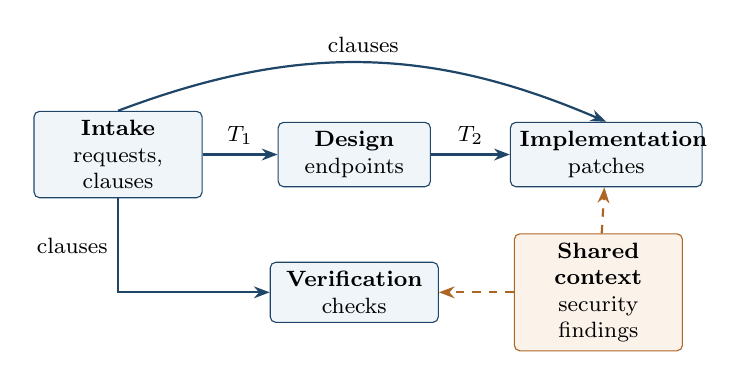
\begin{tikzpicture}[font=\footnotesize]
\node[box,text width=19mm] (r) at (0,0) {\textbf{Intake}\\requests, clauses};
\node[box,text width=17mm] (d) at (3.0,0) {\textbf{Design}\\endpoints};
\node[box,text width=22mm] (i) at (6.2,0) {\textbf{Implementation}\\patches};
\node[box,text width=19mm] (t) at (3.0,-1.75) {\textbf{Verification}\\checks};
\node[box,text width=19mm,fill=resultamber!10,draw=resultamber!80!black] (c) at (6.1,-1.75) {\textbf{Shared context}\\security findings};
\draw[arr] (r)--node[above]{$T_1$}(d);
\draw[arr] (d)--node[above]{$T_2$}(i);
\draw[arr] (r.south)|-node[pos=0.25,left]{clauses}(t.west);
\draw[arr] (r.north) to[bend left=22] node[above]{clauses}(i.north);
\draw[arr,dashed,draw=resultamber!80!black] (c)--(i);
\draw[arr,dashed,draw=resultamber!80!black] (c)--(t);
\end{tikzpicture}
\caption{Running example. Solid arrows are declared source dependencies; $T_1$ derives an endpoint per request and $T_2$ a patch per endpoint. Dashed arrows carry selected shared context. The controller creates objects and references; agents propose only primitive attribute values (signature text, patch body, check oracle).}\label{fig:network}
\end{figure}

In the terms of this section, the four boxes in Fig.~\ref{fig:network} are views, and $T_1$ and $T_2$ are transformation rules. The controller creates one endpoint per accepted request and one patch per endpoint, together with their references and traces. The jobs are the primitive slots inside these objects: an endpoint's signature text, a patch body and a check's oracle. Each job is filled by the agent that owns its view. The footprint of a patch job contains its endpoint's signature and the clause the patch implements. The context selected for it contains the security findings for that endpoint. Its contract includes the coding instruction and the patch validator.

\subsection{Coordination Failures}\label{sec:failures}
The workflow above admits four failure classes that per-answer checks cannot exclude.
\begin{itemize}
\item[\textbf{F1}] \emph{Stale reply.} A request is sent while the clause has revision~1, the clause changes to revision~2, and the old reply then arrives. It is syntactically valid and may even pass the old tests.
\item[\textbf{F2}] \emph{Local validity, global inconsistency.} The design agent chooses string identifiers and the verification agent integer identifiers. Both outputs pass their local validators.
\item[\textbf{F3}] \emph{Unsafe change of team or rules.} A reviewer is added, a worker's permission is revoked, or a prompt or validator changes. Old evidence is then reused, or old completion verdicts are kept, as if nothing had changed.
\item[\textbf{F4}] \emph{Unbounded or wasted generation.} A failing request is retried on every scheduler pass. Conversely, an unrelated edit causes every artifact to be regenerated.
\end{itemize}

\subsection{Requirements}\label{sec:requirements}
A coordinator for untrusted generative agents should satisfy the following requirements. Section~\ref{sec:guarantees} answers each with a theorem.
\begin{itemize}
\item[\textbf{R1}] \emph{Structural integrity.} Artifact objects, traces and references are well typed and have exactly one producer, whatever the agents return.
\item[\textbf{R2}] \emph{Currentness.} A value is usable only if it was validated against the \emph{current} inputs, contract and owner. Obsolete and duplicate replies cannot write (F1, F3).
\item[\textbf{R3}] \emph{Honest completion.} Publication requires that no work is pending or dirty and that all joint constraints hold (F2, F3).
\item[\textbf{R4}] \emph{Locality.} A change invalidates exactly the work whose inputs changed, not more and not less (F4).
\item[\textbf{R5}] \emph{Bounded effort and termination.} Generation attempts are bounded, and a stable workflow ends in an explicit success or failure verdict (F4).
\item[\textbf{R6}] \emph{Safe reconfiguration.} Changing agents, rules, permissions or validators preserves R1--R3 (F3).
\end{itemize}

% =====================================================================
\section{Approach Overview}\label{sec:overview}

\subsection{Design Principles}
The approach rests on four principles.
\begin{enumerate}
\item \emph{Agents propose, the controller disposes.} Agents never create objects, references or completion verdicts. They return a primitive value for a slot that the controller created, and the controller decides what happens to it.
\item \emph{Depend on exactly what was observed.} Each slot's request is built from an explicit \emph{observation}: the source data, selected context and contract that the agent may see. Its exact encoding, the signature, is the slot's dependency key.
\item \emph{Commit atomically and only if current.} The check ``is this reply still the answer to the current question?'' and the write are a single transaction.
\item \emph{Separate accepted, usable and publishable.} An accepted value may become outdated after an edit. It remains as history, but consumers may read only \emph{usable} values. Release happens only through a global \emph{publication barrier}.
\end{enumerate}

\begin{figure*}[!t]
\centering
\colorlet{inkblue}{black}\colorlet{pale}{gray!12}\colorlet{resultamber}{gray}% grayscale figure
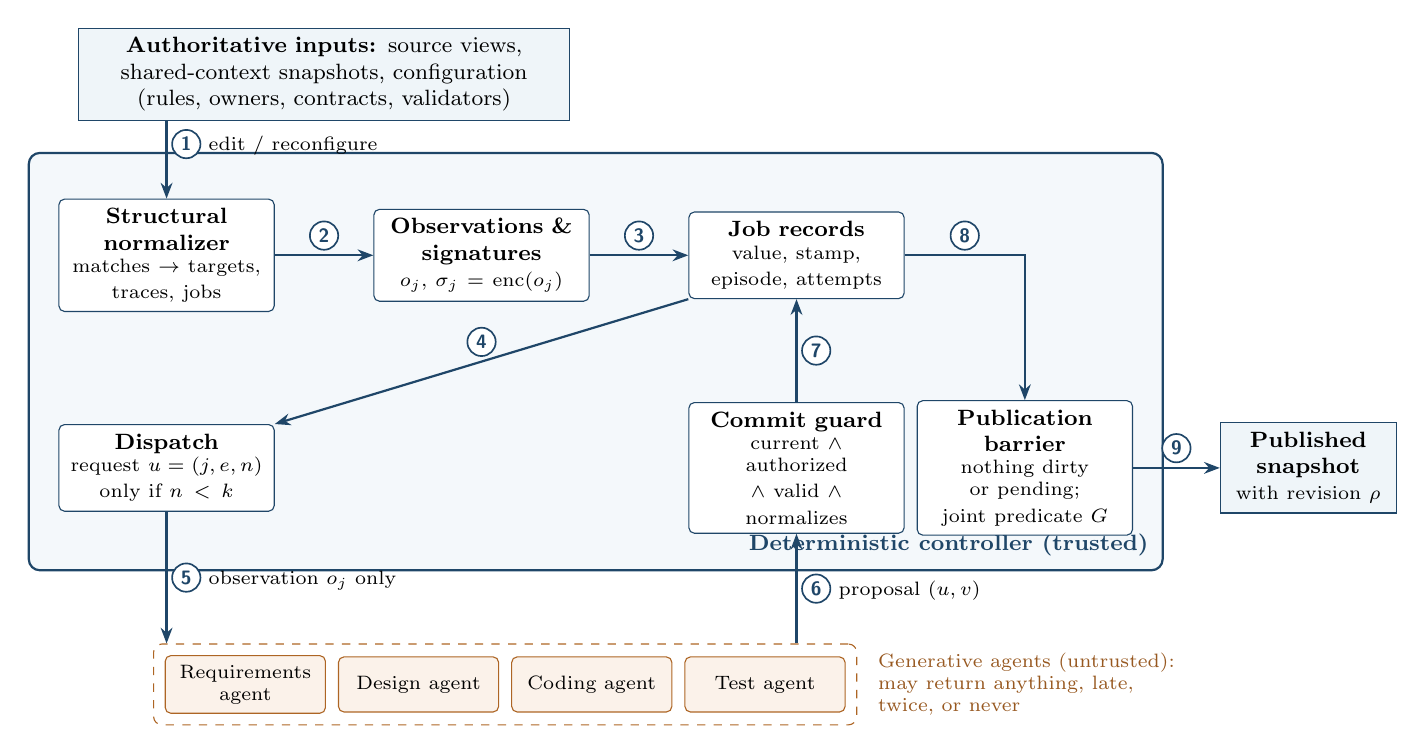
\begin{tikzpicture}[font=\footnotesize,
  comp/.style={draw=inkblue,rounded corners=2pt,fill=white,align=center,minimum height=11mm,text width=25mm},
  agent/.style={draw=resultamber!80!black,fill=resultamber!10,rounded corners=2pt,align=center,text width=18mm,minimum height=7mm,font=\scriptsize},
  lab/.style={font=\scriptsize,align=left,inner sep=1.5pt}]
\node[draw=inkblue,thick,rounded corners=4pt,fill=pale!70,minimum width=14.4cm,minimum height=5.3cm] (ctrl) at (7.35,0.0) {};
\node[anchor=south east,font=\footnotesize\bfseries,text=inkblue] at ([xshift=-2pt,yshift=2pt]ctrl.south east) {Deterministic controller (trusted)};
\node[comp] (norm) at (1.9,1.35) {\textbf{Structural normalizer}\\\scriptsize matches $\to$ targets,\\traces, jobs};
\node[comp] (obs) at (5.9,1.35) {\textbf{Observations \&}\\\textbf{signatures}\\\scriptsize $o_j$, $\Sig_j=\operatorname{enc}(o_j)$};
\node[comp] (rec) at (9.9,1.35) {\textbf{Job records}\\\scriptsize value, stamp,\\episode, attempts};
\node[comp] (disp) at (1.9,-1.35) {\textbf{Dispatch}\\\scriptsize request $u=(j,e,n)$\\only if $n<k$};
\node[comp] (guard) at (9.9,-1.35) {\textbf{Commit guard}\\\scriptsize current $\wedge$ authorized\\$\wedge$ valid $\wedge$ normalizes};
\node[comp] (pub) at (12.8,-1.35) {\textbf{Publication barrier}\\\scriptsize nothing dirty or pending;\\joint predicate $G$};
\node[draw=inkblue,fill=pale,align=center,text width=60mm,minimum height=8mm] (inp) at (3.9,3.65) {\textbf{Authoritative inputs:} source views, shared-context snapshots, configuration (rules, owners, contracts, validators)};
\node[draw=inkblue,fill=pale,align=center,text width=20mm,minimum height=11mm] (snap) at (16.4,-1.35) {\textbf{Published}\\\textbf{snapshot}\\\scriptsize with revision $\rho$};
\node[agent] (a1) at (2.9,-4.1) {Requirements agent};
\node[agent] (a2) at (5.1,-4.1) {Design agent};
\node[agent] (a3) at (7.3,-4.1) {Coding agent};
\node[agent] (a4) at (9.5,-4.1) {Test agent};
\begin{scope}[on background layer]
\node[draw=resultamber!80!black,dashed,rounded corners=3pt,fit=(a1)(a4),inner sep=4pt] (agents) {};
\end{scope}
\node[anchor=west,font=\scriptsize,text=resultamber!70!black,align=left] at ([xshift=4pt]agents.east) {Generative agents (untrusted):\\may return anything, late,\\twice, or never};
\draw[arr] (inp.south -| norm) -- node[lab,right,pos=0.3]{\step{1} edit / reconfigure}(norm.north);
\draw[arr] (norm) -- node[lab,above]{\step{2}}(obs);
\draw[arr] (obs) -- node[lab,above]{\step{3}}(rec);
\draw[arr] (rec.south west) -- node[lab,above,pos=0.5]{\step{4}}(disp.north east);
\draw[arr] (disp.south) -- node[lab,right,pos=0.5]{\step{5} observation $o_j$ only}(disp.south |- agents.north);
\draw[arr] (guard.south |- agents.north) -- node[lab,right,pos=0.5]{\step{6} proposal $(u,v)$}(guard.south);
\draw[arr] (guard.north) -- node[lab,right]{\step{7}}(rec.south);
\draw[arr] (rec.east) -| node[lab,above,pos=0.25]{\step{8}}(pub.north);
\draw[arr] (pub.east) -- node[lab,above]{\step{9}}(snap.west);
\end{tikzpicture}
\caption{Architecture of guarded coordination. Agents (bottom) receive only a declared observation and return a primitive proposal. Everything else, including structure, dependency signatures, attempt budgets, acceptance and publication, belongs to the deterministic controller. Numbered steps are explained in Section~\ref{sec:walkthrough}: (1)~input change, (2)~structural normalization, (3)~signature comparison, (4)~dirty job with budget left, (5)~dispatch, (6)~proposal, (7)~guarded commit or rejection, (8)~usability check, (9)~publication.}\label{fig:overview}
\end{figure*}

\subsection{Walk-Through of One Change}\label{sec:walkthrough}
Fig.~\ref{fig:overview} shows the architecture. We follow the tightened 409 clause through it; Fig.~\ref{fig:sequence} shows the same run as a message sequence, including a stale reply.
\begin{steps}
\item[\step{1}] An authorized editor changes the clause. Every input change and every configuration change is one atomic controller transaction.
\item[\step{2}] The \emph{structural normalizer} recomputes matches of the transformation rules (``one endpoint per accepted request'', ``one patch per endpoint''). It creates or deletes target objects and their traces. Here no object changes, because the request still exists.
\item[\step{3}] For each generated slot, called a \emph{job}, the controller recomputes the observation, meaning the exact data the agent will see. The patch job's observation contains the endpoint signature \emph{and} the clause text, so its signature changes. An unrelated request's jobs keep their signatures and their accepted values remain usable.
\item[\step{4}] A job whose signature changed starts a new \emph{episode} with a fresh attempt budget, and any request still in flight for the old episode is cancelled. Jobs whose prerequisites are unusable are suspended rather than dispatched.
\item[\step{5}] The controller dispatches a request with a fresh identity $u=(j,e,n)$ (job, episode, attempt). The agent receives only the observation and the static instruction.
\item[\step{6}] The agent returns a proposal, perhaps late, perhaps twice, perhaps malformed.
\item[\step{7}] The \emph{commit guard} checks, inside one transaction, that $u$ is still active, that the signature recorded in $u$ equals the job's current signature, that the owner is still authorized, that the validator accepts the value, and that the resulting structure normalizes. Only then does the value become \emph{usable}. The stale reply in Fig.~\ref{fig:sequence} fails the first two checks and is discarded.
\item[\step{8}] The \emph{publication barrier} releases a snapshot only if no required stage is suspended, no job is dirty or pending, and the global predicate $G$ holds. For example, $G$ requires that design and verification agree on the identifier type (F2). Publication \step{9} installs the snapshot with its revision.
\end{steps}

\begin{figure}[!t]
\centering
\colorlet{inkblue}{black}\colorlet{pale}{gray!12}\colorlet{resultamber}{gray}% grayscale figure
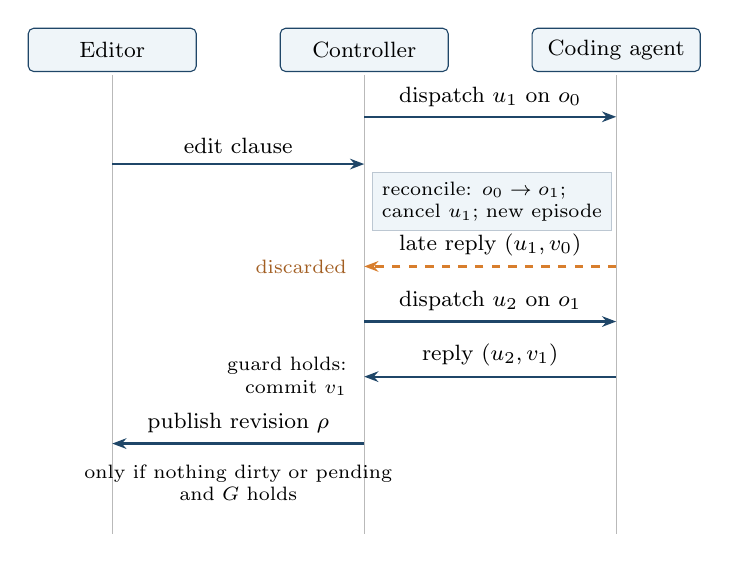
\begin{tikzpicture}[font=\footnotesize,
  msg/.style={-{Stealth[length=1.8mm]},thick,draw=inkblue},
  bad/.style={-{Stealth[length=1.8mm]},thick,draw=resultamber,dashed}]
\foreach \x/\n in {0/Editor,3.2/Controller,6.4/Coding agent} {
  \node[box,text width=19mm,minimum height=5.5mm] at (\x,0) {\n};
  \draw[gray!55] (\x,-0.32) -- (\x,-6.15);}
\draw[msg] (3.2,-0.85) -- node[above]{dispatch $u_1$ on $o_0$} (6.4,-0.85);
\draw[msg] (0,-1.45) -- node[above]{edit clause} (3.2,-1.45);
\node[anchor=north west,align=left,font=\scriptsize,fill=pale,draw=inkblue!30] at (3.3,-1.55) {reconcile: $o_0\to o_1$;\\cancel $u_1$; new episode};
\draw[bad] (6.4,-2.75) -- node[above]{late reply $(u_1,v_0)$} (3.2,-2.75);
\node[anchor=east,font=\scriptsize,text=resultamber!75!black] at (3.1,-2.75) {discarded};
\draw[msg] (3.2,-3.45) -- node[above]{dispatch $u_2$ on $o_1$} (6.4,-3.45);
\draw[msg] (6.4,-4.15) -- node[above]{reply $(u_2,v_1)$} (3.2,-4.15);
\node[anchor=east,align=right,font=\scriptsize] at (3.1,-4.15) {guard holds:\\commit $v_1$};
\draw[msg] (3.2,-5.0) -- node[above]{publish revision $\rho$} (0,-5.0);
\node[anchor=north,font=\scriptsize,align=center,text width=40mm] at (1.6,-5.15) {only if nothing dirty or pending\\and $G$ holds};
\end{tikzpicture}
\caption{Failure F1 handled by the controller. The edit cancels request $u_1$; its late reply cannot commit even if it passes the old validator. If the clause later reverts to $o_0$, a new episode starts and $u_1$ remains cancelled.}\label{fig:sequence}
\end{figure}

\subsection{Key Concepts}
Table~\ref{tab:glossary} defines the vocabulary used in the rest of the paper. Plain-language meanings come first; the formal objects follow in Section~\ref{sec:semantics}.

\begin{table}[!t]
\centering
\caption{Key concepts and notation}\label{tab:glossary}
\footnotesize\setlength{\tabcolsep}{3pt}
\begin{tabular}{@{}>{\raggedright\arraybackslash}p{15mm}>{\raggedright\arraybackslash}p{8mm}>{\raggedright\arraybackslash}p{57mm}@{}}\toprule
Concept & Sym. & Meaning\\\midrule
View & -- & A typed model graph (e.g., the design model) with stable object identities.\\
Rule, match & $r,q$ & A transformation rule and one match of it; $q$ identifies the target object it creates.\\
Job & $j$ & A pair $(q,b)$: one generated primitive attribute $b$ of the target of match $q$, e.g., a patch body.\\
Footprint & $F_j$ & The source data a job's agent may read.\\
Observation & $o_j$ & Footprint, selected context and contract identity $\eta_j$: everything the job depends on.\\
Signature & $\Sig_j$ & Exact injective encoding $\operatorname{enc}(o_j)$; the job's dependency key.\\
Stamp & $a$ & The signature against which the current accepted value was validated.\\
Episode & $e$ & A maximal period with one signature; carries an attempt counter $n\le k$.\\
Request & $u$ & One dispatched generation call, identified by $(j,e,n)$ and never reused.\\
Usable & $U_j$ & Accepted, stamp equals current signature, and all prerequisites usable.\\
Publishable & $\mathit{Pub}$ & Normal form, nothing suspended, dirty or pending, and global predicate $G$ true.\\
Contract & $\eta_j$ & Identity of instruction, schema, validator, environment and generation settings.\\\bottomrule
\end{tabular}
\end{table}

% =====================================================================
\section{Formal Semantics}\label{sec:semantics}
We model the controller as a labeled transition system $(\mathcal S,\mathcal S_0,\Lambda,\to)$ with states $\mathcal S$, initial states $\mathcal S_0$, event labels $\Lambda$ and a transition relation. An \emph{invariant} holds initially and is preserved by every transition. Signatures, identities and primitive values are unbounded, so the system is infinite-state. Diagrams such as Fig.~\ref{fig:automaton} are therefore automaton \emph{schemas}, not claims that the workflow is a finite-state machine. For safety, the proposal source is fully nondeterministic: it may return any value, malformed data, duplicates, or nothing. This over-approximates every possible LLM behavior and needs no probability assumptions.

\subsection{Views, Rules and the Structural Kernel}
Views and metamodels are as in Definition~\ref{def:view}. Let $X$ denote the authoritative source views together with immutable shared-context snapshots. Collection membership, object existence and the absence of a context item are observable data: a dependency analysis that looked only at existing attribute values would miss additions and deletions.

A configuration $C$ contains view metamodels, transformation rules, ownership permissions, context-selection policies, validators, generation contracts and a global predicate $G$. Reads are \emph{ranked} (assumption A0 in Table~\ref{tab:assumptions}): rule matches, structural expressions, observations, selectors and validators read only external data or strictly earlier stages. A \emph{stage} groups independent rules processed after their prerequisites.

A rule has a tuple source pattern, a deterministic guard, one target object, deterministic structural bindings, and zero or more generated primitive bindings. A match is identified by the key $q=(r,\operatorname{id}(s_1),\ldots,\operatorname{id}(s_m))$, such as $(\mathsf{RequestToEndpoint},\mathsf{request17})$. A deterministic injective constructor yields the target identity $\iota(q)$ and the persistent trace $q\mapsto\iota(q)$. Producers use disjoint identifier namespaces. A reference resolves through traces only if the referenced match exists; a missing mandatory target makes normalization fail rather than leaving a dangling reference.

The \emph{structural normalizer} $N_C$ maps a coherent view snapshot to an internal skeleton. It computes the current match set, creates missing targets, removes obsolete targets and their traces, and computes deterministic attributes and references. It keeps accepted generated values only for surviving bindings whose contract remains compatible. Generated slots that have no value yet hold $\nodata$. $N_C$ is partial: inadmissible candidate snapshots are rejected.

\begin{definition}[Structural admissibility]\label{def:struct}
Configuration $C$ is \emph{structurally admissible} on a snapshot if $N_C$ terminates, is deterministic and idempotent, produces exactly one owned target and trace per match key, creates only well-typed references, and satisfies all multiplicity constraints. Generated bindings may write only declared primitive slots, and every write has exactly one configured owner.
\end{definition}

Admissibility is a proof obligation for a concrete transformation engine, not a property of arbitrary transformation programs. A simple sufficient construction allocates all targets first and resolves references second, a separation familiar from ATL~\cite{atl}.

\begin{theorem}[Constructive structural kernel]\label{thm:kernel}
Consider finite source graphs and finitely many single-target rules whose guards and structural expressions are pure and terminating. Suppose target identities $\iota(q)$ are injective, producer namespaces are disjoint, primitive expressions have declared types, and each reference expression returns a finite set of current match keys of the required target type and multiplicity. Then enumerating matches, allocating all targets, and resolving references constructs an admissible skeleton. The result is unique, and idempotent when generated slots are held fixed.
\end{theorem}
\begin{proof}
Each source product is finite, so terminating guards yield a finite match set. Allocation creates one target per key; injectivity and disjoint namespaces exclude collisions, and the trace is exactly the graph of $\iota$ on that set. Each reference key lies in this domain by hypothesis, so second-phase lookup succeeds and preserves type and cardinality. Typed primitive expressions preserve attribute types. Purity makes the match set and structural values independent of enumeration order, which gives uniqueness. Repeating the construction yields the same keys, identities, references and values, which gives idempotence. Deleting targets outside the current key set yields exact coverage, and all references are recomputed in the same transaction. Induction over the finite rank order extends the argument to all enabled stages.
\end{proof}

If a prerequisite stage is unavailable, its dependent stage is \emph{suspended}: it contributes no active targets, traces or jobs, and old accepted values are kept only in a private cache that consumers cannot read. A set $Q$ records suspended required stages, so an empty job set is never mistaken for completion. On reactivation, stable keys reconstruct the objects, and cached values are restored only if observation, contract and authority are compatible.

\subsection{Observations and Dependency Signatures}
A job $j=(q,b)$ is one generated attribute $b$ of the target of match $q$. Let $Z$ be the coherent readable snapshot formed from $X$ and the currently usable generated predecessors, built in rank order. The job's \emph{effective observation} is
\begin{equation}\label{eq:obs}
o_j=\obs_{C,j}(Z)=\bigl(F_j(Z),\ \operatorname{select}_{C,j}(Z),\ \eta_{C,j}\bigr),
\end{equation}
where $F_j$ is a pure, total source-footprint expression, $\operatorname{select}_{C,j}$ returns the authorized context items (including explicit absence markers), and $\eta_{C,j}$ identifies the generation and validation contract: instruction, schema, validator and its environment, source expression, selection policy and generation settings. A configuration change need not invalidate every job, but it must change $\eta$ for every job it affects.

The \emph{signature} $\Sig_j=\operatorname{enc}(o_j)$ is an injective canonical encoding, so different observations never share an encoding. In the mathematics it is exact equality. An implementation may store the encoding or use a digest with collision detection; a bare cryptographic digest makes the results conditional on the absence of collisions. Context version numbers enter $o_j$ only if the agent or validator actually sees them. Otherwise, equal selected content at different versions has equal signatures, and no regeneration is needed (scenario S10 in Section~\ref{sec:rq3}).

A footprint describes a dependency \emph{function}, not merely the locations visited last time. The query ``all findings for endpoint $e$'' depends on the membership of that set as well as on its contents, so adding a matching finding must change the observation (scenario S09). Unavailable or access-denied context yields $o_j=\nodata$ and blocks dispatch; silently substituting empty text would change the contract.

\begin{definition}[Footprint adequacy, validator soundness]\label{def:adequate}
Let $R_j(Z,v)$ be the desired domain relation between snapshots and proposed values. A footprint is \emph{adequate} for $R_j$ if there is $\widehat R_j$ with $R_j(Z,v)=\widehat R_j(o_j,v)$ for all admissible $Z,v$. A validator $V_j(o,v)$ is \emph{sound} for $R_j$ if $V_j(o,v)\Rightarrow\widehat R_j(o,v)$.
\end{definition}

Informally, two snapshots with the same observation must yield the same validity judgment for any proposal. Adequacy is a semantic obligation; signature equality is a mechanical test. A footprint containing only the endpoint signature is \emph{not} adequate for the 409 clause, because two snapshots may have equal signatures and different clauses. No freshness mechanism can repair an inadequate footprint.

\subsection{Controller State and the Job Automaton}
The controller state is $S=(C,X,Y,L,B,P,A,H,Q,\nu,\rho)$: configuration, authoritative inputs, active skeleton, traces, job records, active requests, immutable history and evidence, published snapshot, suspended required stages, a monotone nonce allocator and a semantic revision counter. A job record holds an accepted triple $(v,a,\gamma)$ (value, stamp, evidence pointer) or none, a failed signature $f$ or none, an episode nonce $e$, the episode signature $s$, and an attempt counter $n\in\{0,\ldots,k\}$ for a fixed budget $k\ge1$. An episode is a maximal period during which an active job keeps one signature. Returning to an earlier signature, or reactivating a suspended job, starts a \emph{new} episode. Nonces are allocated monotonically, so a request identity $u=(j,e,n)$ is never reused, even after deletion and recreation of the job. The history $A$ retains every dispatched request, which lets late and duplicate deliveries be recognized.

For an active job, freshness, usability and the set of outstanding obligations are defined in rank order:
\begin{align}
\fresh_j(S)&\iff B_j\text{ holds }(v,a,\gamma)\ \land\ a=\Sig_j(S),\label{eq:fresh}\\
U_j(S)&\iff j\text{ active}\land\fresh_j(S)\land\textstyle\bigwedge_{i\prec j}U_i(S),\label{eq:usable}\\
O(S)&=\{j\in\Jobs(S):\neg U_j(S)\}.\label{eq:obligation}
\end{align}
Here $i\prec j$ ranges over declared generated prerequisites. Downstream consumers read a value only through the $U_j$ gate. If an upstream value becomes unusable, all its descendants become unusable too, even if their old bytes are still stored. Validators are total and deterministic on their declared observations; validators that call external tools must include tool versions in the contract.

Fig.~\ref{fig:automaton} summarizes a job's control states, which are derived from the record. A dependency change cancels pending authority and starts a new episode. The job is then Dirty, unless compatible cached evidence immediately makes it Fresh again (for example, after reversion to an earlier observation). Failed is terminal for an unchanged episode but is not a successful state. No agent can move a job directly to Fresh.

\begin{figure}[!t]
\centering
\colorlet{inkblue}{black}\colorlet{pale}{gray!12}\colorlet{resultamber}{gray}% grayscale figure
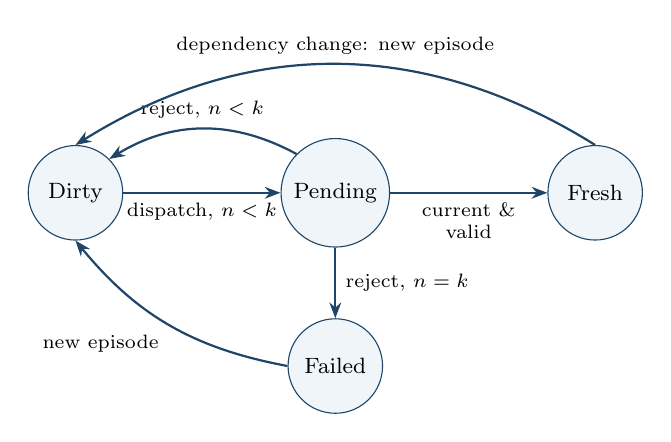
\begin{tikzpicture}[>=Stealth,every state/.style={draw=inkblue,fill=pale,font=\footnotesize,minimum size=12mm}]
\node[state] (d) at (0,0) {Dirty};
\node[state] (p) at (3.3,0) {Pending};
\node[state] (f) at (6.6,0) {Fresh};
\node[state] (e) at (3.3,-2.2) {Failed};
\draw[arr] (d) -- node[below,font=\scriptsize]{dispatch, $n<k$}(p);
\draw[arr] (p) -- node[below,font=\scriptsize,align=center]{current \&\\valid}(f);
\draw[arr] (p.north west) to[bend right=30] node[above,font=\scriptsize]{reject, $n<k$}(d.north east);
\draw[arr] (p)--node[right,font=\scriptsize]{reject, $n=k$}(e);
\draw[arr] (f.north) to[bend right=32] node[above,font=\scriptsize]{dependency change: new episode}(d.north);
\draw[arr] (e.west) to[bend left=20] node[below left,font=\scriptsize]{new episode}(d.south);
\end{tikzpicture}
\caption{Control automaton schema of one job. A dependency change cancels pending authority and starts a new episode (shown here from Fresh). Compatible cached evidence can restore Fresh directly. Obsolete replies never cause a transition.}\label{fig:automaton}
\end{figure}

\subsection{Transition Rules}\label{sec:rules}
Every transition is one atomic controller transaction; Table~\ref{tab:rules} lists them. Two rules deserve comment.

\emph{Resolve.} For a returned pair $(u,v)$, let $\Sig_u$ and $o_u$ be the signature and observation recorded in request $u$. The commit guard requires that $u$ is active in $P$, that it belongs to the same job and episode, that its owner is still authorized, that all prerequisites are usable, that the value has the slot's primitive type, and that
\begin{equation}\label{eq:guard}
\Sig_u=\Sig_j(S),\qquad o_j(S)\ne\nodata,\qquad V_j(o_u,v).
\end{equation}
Because a generated attribute may influence later matches or references, the value is first installed in a private \emph{candidate} state, on which complete downstream normalization and reconciliation run. The candidate is committed only if every enabled structural check succeeds; otherwise the attempt counts as failed. The equality test and the write must share one linearization point~\cite{herlihy1990linearizability} with edits and reconfigurations. Validation may run outside the transaction on the immutable $o_u$, but its result counts only after the guard is rechecked inside the transaction. This is optimistic concurrency control~\cite{occ}.

\emph{Publish.} Let $G$ be a total predicate over an immutable candidate snapshot that encodes all joint constraints and required executable checks. Then
\begin{equation}\label{eq:publish}
\begin{split}\Pub(S)\iff{}&\text{normal form}\land Q=\emptyset\land O(S)=\emptyset\\&{}\land P=\emptyset\land G(C,X,Y,B,L).\end{split}
\end{equation}
Only a Publish transition satisfying~\eqref{eq:publish} installs $H$, with that exact snapshot and revision. Later edits leave $H$ as a historical snapshot but remove any claim that it represents the current state.

\begin{table*}[!t]
\centering
\caption{Controller transitions (concrete machine) and their counterparts in the atomic specification used for refinement (Theorem~\ref{thm:refinement}). Unmentioned components are unchanged; $\mathcal R$ is rank-order normalization and reconciliation.}\label{tab:rules}
\footnotesize\setlength{\tabcolsep}{4pt}
\begin{tabular}{@{}P{22mm}P{64mm}P{58mm}P{22mm}@{}}\toprule
Transition & Guard & Effect & Abstract action\\\midrule
Edit / Normalize & Authorized edit; candidate passes $N_C$ & Install input; apply $\mathcal R$: new episodes for changed signatures, cancel their requests, suspend unavailable stages; advance $\rho$. On failure keep state, record rejection. & Edit\\
Dispatch$(j)$ & $j\in O(S)$; $o_j\ne\nodata$; prerequisites usable; no active request; $f\ne\Sig_j$; $n<k$ & $n\gets n+1$; record request $(u,j,e,\Sig_j,o_j)$ and owner in $P$ and $A$; send only $o_j$ and static instruction & Attempt (budget increment)\\
Resolve (commit) & $u\in P$; same job/episode; owner authorized; Eq.~\eqref{eq:guard}; type check; candidate normalizes & Install $(v,\Sig_u,\gamma)$; clear $f$; remove $u$; apply $\mathcal R$; advance $\rho$ & Accept\\
Resolve (reject) / Timeout & $u\in P$ current, but validation, typing or normalization fails, or timeout & Remove $u$; if $n=k$ set $f\gets\Sig_j$ & Fail\\
Discard & $u\notin P$, obsolete or unauthorized & None (duplicate or late delivery) & Stutter\\
Publish & Eq.~\eqref{eq:publish} on an immutable snapshot & Install $H$ with that snapshot and revision & Publish (without $P=\emptyset$)\\
Reconfigure & Candidate $C'$ admissible, ownership and policy compatible, satisfies A0 (and A5 if progress is required) & Install $C'$; apply $\mathcal R$; migrate compatible records; cancel requests whose job, authority or contract changed; advance $\rho$ & Reconfigure\\\bottomrule
\end{tabular}
\end{table*}

\subsection{Assumptions}
Table~\ref{tab:assumptions} collects the assumptions used by the guarantees. They are independent: disjoint ownership protects writes, exact signatures protect dependency comparison, and sound validation connects acceptance to a domain property. None implies another.

\begin{table}[!t]
\centering
\caption{Assumptions and the guarantees that require them}\label{tab:assumptions}
\footnotesize\setlength{\tabcolsep}{3pt}
\begin{tabular}{@{}lP{50mm}l@{}}\toprule
ID & Assumption & Used for\\\midrule
A0 & Finite ranked read dependencies; unavailable stages are suspended & Well-defined semantics\\
A1 & Admissible deterministic normalizer; agents write primitives only & Structure\\
A2 & Exact effective signatures; every relevant contract change alters $\eta$ & Currentness, locality\\
A3 & Linearizable controller transactions; immutable observations & Commit safety\\
A4 & Total validators over recorded observations; stable declared environment & Acceptance\\
A5 & Finite acyclic dependency graph, single producers, stage stability & Termination\\
A6 & Inputs and configuration stabilize; fair controller; requests settle & Progress\\
A7 & Adequate footprints; sound local and global validators & Domain correctness\\\bottomrule
\end{tabular}
\end{table}

% =====================================================================
\section{Guarantees}\label{sec:guarantees}
This section states and proves the guarantees, organized by the requirements of Section~\ref{sec:requirements}. Table~\ref{tab:evidence} at the end summarizes each guarantee with its assumptions and supporting evidence.

\subsection{Safety (R1--R3)}
A committed value need not remain fresh after an edit; the controller must instead prevent its \emph{use} until it is repaired. We therefore distinguish a historical acceptance invariant from current usability. Claiming that every stored value is always fresh would be false in exactly the change scenarios of interest.

\begin{theorem}[Controller safety]\label{thm:safety}
Under A0--A4, from a normalized initial state with no accepted values, every reachable state satisfies:
(i) active targets and traces have unique producers and valid structural references;
(ii) each accepted record carries evidence of an authorized successful validation against its recorded observation and contract;
(iii) every usable value satisfies the current validator for the current observation;
(iv) every committed reply was current and authorized at its commit linearization point; and
(v) every installed published snapshot satisfied~\eqref{eq:publish} at installation.
\end{theorem}
\begin{proof}
By induction on run length. Initially, (i) holds by A1 and the other claims are vacuous. \emph{Edit} preserves (i) by A1. It keeps acceptance evidence only as history and recomputes usability, so a changed observation cannot make an old value usable unless observation and contract agree exactly. \emph{Dispatch} changes no accepted value or structure. A successful \emph{Resolve} writes the owned slot in a candidate and normalizes the dependent structure before admitting it; Theorem~\ref{thm:kernel} or A1 gives (i) for the new graph, and a rejected candidate changes nothing. Request identity and authorization give the provenance part of (ii); the validator and exact-signature tests give (iii) and (iv). Failed and discarded replies write no accepted value, and timeouts change only attempt state. \emph{Publish} tests the exact snapshot it installs, which gives (v). \emph{Reconfigure} normalizes under the new admissible configuration, invalidates incompatible evidence and cancels obsolete authority, so it preserves (i)--(iv) and never relabels a historical publication as current. In (iii), equality of encoded observations implies equality of validator inputs and contract by A2 and A4.
\end{proof}

\begin{corollary}[Validator-relative domain correctness]\label{cor:domain}
If a usable value $v$ has an adequate footprint and a sound validator (Definition~\ref{def:adequate}), then $R_j(Z,v)$ holds. If $G$ is sound for a desired snapshot relation $R_G$, every published snapshot satisfies $R_G$.
\end{corollary}
\begin{proof}
Theorem~\ref{thm:safety}(iii) gives $V_j(o_j,v)$; soundness gives $\widehat R_j(o_j,v)$; adequacy identifies it with $R_j(Z,v)$. The second claim applies soundness of $G$ to the publication guard.
\end{proof}

\begin{example}[Limits of parsing and test evidence]\label{ex:limits}
A patch that returns 200 for every request may parse and type-check while violating the 409 clause; such a validator is not sound for that clause. A generated test that fails on one empty stub need not detect an incorrect implementation. Locally accepted endpoints with different identifier types can violate a joint interface constraint, which $G$ or a certified cross-binding validator must check. Rejection at the barrier is an honest blocked outcome, not a promise that automatic repair will succeed.
\end{example}

\subsection{Asynchronous Refinement (R2)}
Theorem~\ref{thm:safety} is stated for the concrete, asynchronous controller. We now show that asynchrony adds no behavior beyond an atomic specification. The abstract machine $\mathcal A$ has the same configuration, inputs, structure, accepted records, attempt and failure records, and publication, but no remote requests. Its actions are those in the last column of Table~\ref{tab:rules}. \emph{Accept} may choose any value that satisfies the current observation's validator and ownership condition, provided the candidate normalizes. Let $\alpha(S)$ erase requests and delivery detail while retaining semantic and budget records. Note that concrete dispatch maps to an abstract budget increment, not to a stutter: claiming that dispatch stutters while an incremented counter remains visible would be incorrect.

\begin{theorem}[Forward simulation]\label{thm:refinement}
Under A0--A4, every concrete run projects through $\alpha$ to a run of $\mathcal A$, allowing stuttering. Hence asynchronous replies cannot introduce a value forbidden by the atomic specification.
\end{theorem}
\begin{proof}
We map each concrete transition. Dispatch maps to Attempt, since both increment the same episode budget and request creation is erased. A successful Resolve maps to Accept: the concrete signature test implies that the recorded observation is exactly the current abstract observation, the remaining tests imply the abstract validator and ownership guards, and both use the same candidate normalization. A current rejection or timeout maps to Fail, including the exhaustion mark. Obsolete and duplicate deliveries change no retained record and map to stutters; signature reconciliation belongs to the associated Edit or Reconfigure in both machines. Edit, Reconfigure and Publish use the same normalized snapshots, and concrete Publish has all abstract guards. Initial projections agree, so induction yields a projected run. We do not claim the converse or any liveness correspondence~\cite{lynch1995simulations,abadi1991refinement}.
\end{proof}

The guards are not redundant in general. If both cancellation of obsolete requests and the commit-time signature check are removed, the sequence ``dispatch on $o_0$, edit to $o_1$, deliver the old valid answer'' commits obsolete provenance. Either defense alone suffices in the one-job model. A check-then-write race outside the transaction bypasses both. Without unique request identities, a duplicated reply can overwrite a newer accepted value after deletion and recreation. Section~\ref{sec:rq1} confirms each of these mechanisms experimentally.

\subsection{Locality and Isolation (R4)}
For two normalized snapshots with the same job identities and contract, the \emph{direct impact set} is
\begin{equation}\label{eq:impact}
D(Z,Z')=\{j : o_j(Z)\ne o_j(Z')\}.
\end{equation}
Newly created jobs are dirty and deleted jobs are removed; structural matching is handled separately.

\begin{theorem}[Exact direct invalidation]\label{thm:local}
Assume all surviving jobs are usable before one authorized edit, no job is pending, and no generated value changes during the edit transaction. For each surviving job whose prerequisites remain available, its accepted stamp becomes stale if and only if $j\in D(Z,Z')$. Jobs outside $D$ retain their validator-relative value. Descendants of unusable prerequisites are additionally blocked until those prerequisites are repaired.
\end{theorem}
\begin{proof}
Before the edit, $a_j=\operatorname{enc}(o_j(Z))$; after it the stored value is unchanged and the current signature is $\operatorname{enc}(o_j(Z'))$. Injectivity gives $a_j\ne\Sig_j(Z')$ exactly when $o_j(Z)\ne o_j(Z')$. If the observations agree, validator input and contract agree, so the earlier validation still applies. The prerequisite gate in~\eqref{eq:usable} explains descendant blocking.
\end{proof}

An unchanged upstream output permits \emph{early cutoff}. After an upstream job is repaired to the same value, an observation-equal descendant becomes usable again without regeneration (scenario S16). This is the main source of savings in RQ2. The dependency graph must cover guards, membership queries, structural expressions, validators and selected context as well as prompt text; a graph that omits any of these supports neither locality nor scheduling.

\begin{proposition}[Observation-relative isolation]\label{prop:isolation}
If two states agree on a job's observation, contract, attempt record, request activity, authorization and prerequisite usability, they admit the same dispatch eligibility and the same set of locally valid proposals for that job, even if unselected source or context content differs.
\end{proposition}
\begin{proof}
Every local guard is a function of the listed data, so substituting equals preserves its truth and the validator's accepted-value set.
\end{proof}

This is a statement about the controller's inputs, not information-theoretic confidentiality: pretraining, logs or tool access may reveal more unless they are controlled separately.

\subsection{Bounded Generation (R5)}
Let $E_j$ be the number of signature episodes of job $j$ during a finite interval, counting episodes interrupted by edits, started by reactivation, by a change of $\eta$, or by deletion and recreation.

\begin{theorem}[Generation bound]\label{thm:cost}
For any finite execution interval that starts with fresh episode budgets,
\begin{equation}\label{eq:calls}
N_{\mathrm{dispatch}}\le k\textstyle\sum_j E_j.
\end{equation}
If each request $u$ has at most $p_u$ input tokens and a provider-enforced output cap $\ell_u$, the accounted generation tokens satisfy $T\le\sum_{u}(p_u+\ell_u)$, which is at most $k(p+\ell)\sum_jE_j$ for common caps $p,\ell$.
\end{theorem}
\begin{proof}
Within an episode $n$ starts at zero, dispatch strictly increments it, and no transition decreases it, so the guard $n<k$ allows at most $k$ dispatches. Retries, timeouts and obsolete replies do not reset $n$ within the episode. Summing over episodes gives~\eqref{eq:calls}; summing the per-request caps, including those of discarded requests, gives the token bound.
\end{proof}

The bound charges observed episodes, not distinct signature values: the input sequence $a,b,a,b$ earns four budgets, so continuous editing can cause unbounded work. The simpler bound $k|D|$ holds when each affected job is processed once after its prerequisites stabilize. The theorem bounds generation calls and tokens; it does not bound matching, validation or wall-clock time. A request to ``be brief'' is not an enforced cap.

\subsection{Terminal Outcomes (R5)}
Acyclicity must hold for all data dependencies, not merely for arrows between agent names. Assumption A5 partitions jobs and structural stages into a finite directed acyclic graph. Jobs in one stage are mutually independent, each node has one producer, and no output influences its own or an earlier stage's existence, validation or selection policy. Algorithm~\ref{alg:schedule} processes the stages of one frozen revision in topological order. It retains usable values whose observations are unchanged. Because jobs within a stage are independent, the inner loop over a stage's jobs may run in parallel. A job that is still unusable after the loop is classified as failed, either because it exhausted its budget or because its observation is unavailable. Dependents of failed prerequisites are classified as \emph{blocked} without calling an agent. Blocked is an explicit terminal verdict, not a satisfied requirement.

\begin{algorithm}[!t]
\caption{Topological repair of a stable revision}\label{alg:schedule}
\footnotesize
\begin{algorithmic}[1]
\Require admissible $C$, frozen external revision $X$, budget $k\ge1$
\For{stage $s$ in topological order}
  \If{a required predecessor of $s$ is failed or blocked}
    \State classify $s$ as blocked; \textbf{continue}
  \EndIf
  \State normalize $s$; create/delete jobs; reconcile signatures
  \For{each job $j$ in $s$ with $\neg U_j$}
    \While{$\neg U_j\land n_j<k\land o_j\ne\nodata$}
      \State guarded Dispatch$(j)$
      \State await reply or timeout
      \State guarded Resolve
    \EndWhile
    \If{$\neg U_j$} classify $j$ as failed \EndIf
  \EndFor
\EndFor
\If{$\Pub(S)$}
  \State publish the snapshot
\Else
  \State report failure, blockage or global conflict
\EndIf
\end{algorithmic}
\end{algorithm}

\begin{theorem}[Terminal outcome]\label{thm:termination}
Under A0--A6 and Algorithm~\ref{alg:schedule}, once external input and configuration stabilize, the controller eventually reports either a publishable snapshot or an explicit failure, blockage or global conflict. A new topological pass dispatches at most $k|\Jobs_*|$ requests, where $\Jobs_*$ contains all job instances appearing during the pass. Publication follows if every required observation is available, every dirty job obtains a committed proposal within its budget, and the resulting snapshot satisfies $G$.
\end{theorem}
\begin{proof}
At the first stage external inputs are stable, so normalization produces finitely many jobs. A usable job needs no request. Every other available job either succeeds or exhausts its finite budget, because the controller progresses fairly and every dispatch eventually resolves or times out (A6); unavailable jobs are classified directly. Inductively, the predecessors of each later stage are stable. If one has failed, the stage is blocked; otherwise pure normalization and observations yield a fixed finite job set with fixed signatures, and the same argument applies. Independence within a stage ensures that a sibling cannot change a job's observation. With finitely many stages the global predicate is eventually evaluated. Summing at most $k$ dispatches per instantiated job gives the request bound, and the additional hypotheses exclude every failure case.
\end{proof}

Finite budgets guarantee termination, not successful synthesis. Cyclic dependencies lie outside A0: a Boolean value updated by $v\gets\neg v$ along a feedback edge oscillates forever even though each proposal is locally valid. Convergence for cyclic consistency restoration requires an independent well-founded ranking~\cite{klare,stevens}.

\subsection{Safe Reconfiguration (R6)}
Adding an agent, changing a rule, revoking a permission or replacing a validator is a configuration transformation $h:C\mapsto C'$. Adding a security reviewer, for instance, creates new targets and obligations and extends $G$. Keeping the earlier publication as ``current'' while the reviewer has produced nothing would be incorrect. This is the generative-workflow analogue of safe dynamic change in component systems~\cite{kramer1990evolving,vandewoude2007tranquility}.

\begin{theorem}[Transactional reconfiguration]\label{thm:reconfig}
Let $S$ satisfy the invariant of Theorem~\ref{thm:safety}. A configuration transaction that checks A0--A4 for $C'$, invalidates every changed observation or authority, reconciles structure and jobs, and recomputes completion yields a state that satisfies the invariant under $C'$. If it also preserves A5 and configuration changes eventually stop, Theorem~\ref{thm:termination} applies to the new revision.
\end{theorem}
\begin{proof}
The installed structure is in the range of $N_{C'}$, which gives (i). A retained usable record has the same effective observation and compatible authority, so its evidence still proves (ii)--(iii); every other record is historical or invalidated and cannot pass the usability gate. Requests whose job, contract or authority changed are cancelled, and unchanged ones must still pass the current commit guard, which gives (iv). No historical publication is relabeled current, and any new publication must pass the recomputed predicate, which gives (v). Atomic installation prevents readers from observing mixed configurations.
\end{proof}

Revocation cancels future commitment but cannot recall data already sent to an agent. Rollback and compensation of external side effects need additional protocols.

\subsection{Extensions}\label{sec:extensions}
\emph{Structured ingress.} Natural-language input can enter through a separate \emph{lifting} agent that proposes a typed source delta $\Delta$. Treating $\Delta$ as an untrusted Edit, checked for ownership, types, source invariants and the absence of writes into controller-owned namespaces, preserves Theorem~\ref{thm:safety} unchanged (scenario S27). Fidelity of $\Delta$ to the user's intent needs an explicit relation and a checker or human confirmation.

\emph{Shared writers.} A shared-context update is an authorized Edit with an expected-version check: of two writers starting from version $v$, only the first to commit succeeds (scenario S24). This prevents lost updates but does not resolve semantic disagreement.

\emph{External observation.} Let $W$ hold an outbox and a remote observer's projection. Committed events may be copied into $W$; loss, duplication and delivery affect only $W$. Admission guards and evidence never read $W$, and a failed copy never blocks the controller.

\begin{proposition}[Observational extension]\label{prop:observation}
Erasing $W$ maps every run of the extended system to a run of the controller, allowing stutters, so observer transport cannot falsify the controller's safety invariant.
\end{proposition}
\begin{proof}
An extended controller step has the base step's guard and authoritative effect plus an optional copy into $W$, so it projects to that base step. A pure transport step changes only $W$ and projects to a stutter. Induction transfers safety.
\end{proof}

\subsection{Boundary Cases and Summary}
Table~\ref{tab:boundaries} lists counterexamples that delimit the results. Each identifies a specification or implementation obligation; the last column shows where the evaluation exercises it. Table~\ref{tab:evidence} maps every guarantee to its assumptions and its evidence.

\begin{table}[!t]
\centering
\caption{Counterexamples, the discipline that excludes them, and where the evaluation exercises them (M: TLC mutant; Ab: implementation ablation; S: scenario)}\label{tab:boundaries}
\footnotesize\setlength{\tabcolsep}{3pt}
\begin{tabular}{@{}P{30mm}P{29mm}P{17mm}@{}}\toprule
Counterexample & Required discipline & Exercised\\\midrule
Clause changes, interface signature equal & Adequate footprint (A7) & S03, S17\\
Reply arrives after a source edit & Cancellation or atomic recheck & M, Ab, S11\\
Two locally valid outputs disagree & Global predicate $G$ & Ab, S18\\
Exhausted request retried every pass & Persistent per-episode budget & M, Ab, S14\\
New matching context item added & Membership in footprint & M, Ab, S09\\
Prompt or validator changes, input does not & Contract $\eta$ in signature & M, Ab, S23\\
Revoked owner's reply arrives & Authority in guard & M, Ab, S22\\
Locally valid value breaks structure & Candidate normalization & Ab, S19\\
Value read while its prerequisite is stale & Upstream gate in $U_j$ & Ab, S15\\
Feedback edge flips a value forever & Acyclic schedule (A5) & Theorem~\ref{thm:termination}\\
Old request arrives after recreation & Never-reused request identities & Test T02\\\bottomrule
\end{tabular}
\end{table}

\begin{table*}[!t]
\centering
\caption{Guarantees, assumptions and evidence. $\bullet$: complete for the stated scope; $\circ$: partial or scoped (e.g., a lemma used by the proof, a bounded instance); --: none. \emph{Exec.} denotes executable checks on the reference controller (Section~\ref{sec:evaluation}).}\label{tab:evidence}
\footnotesize\setlength{\tabcolsep}{4pt}
\begin{tabular}{@{}llcccccP{58mm}@{}}\toprule
Guarantee & Requirement & Assumptions & Paper proof & TLAPS & TLC & Exec. & Remaining obligation\\\midrule
Thm.~\ref{thm:kernel} Structural kernel & R1 & -- & $\bullet$ & $\circ$ & -- & $\bullet$ & Connect typed kernel to the full protocol model\\
Thm.~\ref{thm:safety} Controller safety & R1--R3 & A0--A4 & $\bullet$ & $\circ$ & $\circ$ & $\bullet$ & Mechanize the full inductive invariant\\
Cor.~\ref{cor:domain} Domain correctness & R2 & A7 & $\bullet$ & $\circ$ & -- & $\circ$ & Adequacy and soundness beyond the finite language\\
Thm.~\ref{thm:refinement} Forward simulation & R2 & A0--A4 & $\bullet$ & -- & -- & $\circ$ & Checked refinement mapping to the atomic model\\
Thm.~\ref{thm:local} Exact invalidation & R4 & A2 & $\bullet$ & -- & -- & $\bullet$ & Machine proof\\
Prop.~\ref{prop:isolation} Isolation & R4 & A2 & $\bullet$ & -- & -- & $\circ$ & --\\
Thm.~\ref{thm:cost} Generation bound & R5 & A3 & $\bullet$ & $\circ$ & $\circ$ & $\bullet$ & History-counting induction across episodes\\
Thm.~\ref{thm:termination} Terminal outcome & R5 & A0--A6 & $\bullet$ & -- & $\circ$ & $\circ$ & Unbounded temporal mechanization\\
Thm.~\ref{thm:reconfig} Reconfiguration & R6 & A0--A5 & $\bullet$ & -- & $\circ$ & $\bullet$ & Parameterized preservation proof\\
Prop.~\ref{prop:observation} Observation & R3 & A3 & $\bullet$ & -- & -- & $\circ$ & No completeness/authenticity of remote timelines\\
Thm.~\ref{thm:table} Policy table & R2 & A7 & $\bullet$ & $\circ$ & -- & $\bullet$ & Refinement of the Python interpreter\\\bottomrule
\end{tabular}
\end{table*}

% =====================================================================
\section{Instantiation}\label{sec:instantiation}

\subsection{Document-Service Case Study}\label{sec:case-study}
The executable case study instantiates the running example as a ranked chain of four views per source document: requirements, architecture, implementation and verification. A fifth security-review view can be added at run time. Each view has one stable target and one generated JSON attribute per document (Table~\ref{tab:bindings}). The three requirements are as follows. R01 requires stable string document identities. R02 specifies the exact lifecycle behavior (state and status). R03 requires complete view metadata and matching identifier types in architecture and verification.

Two choices make the case study deliberately adversarial. First, the architecture validator \emph{locally} accepts either a string or an integer identifier type, but the downstream structural expression requires strings. An integer proposal is therefore locally valid yet must be rejected by candidate normalization (failure F2 at the structural level). Second, verification may also choose an integer type independently, which only the global predicate catches (F2 at the publication level).

\begin{table}[!t]
\centering
\caption{Case-study bindings, their observations and validator strength}\label{tab:bindings}
\footnotesize\setlength{\tabcolsep}{3pt}
\begin{tabular}{@{}lP{26mm}P{30mm}@{}}\toprule
View & Observation (inputs) & Local validator\\\midrule
Requirements & Source policy & Clause IDs; exact Boolean policy\\
Architecture & Usable requirements & Operation list; typed ID choice (string or integer)\\
Implementation & Interface, clause, selected findings & \emph{Sound and complete}: exact six-row policy table (Thm.~\ref{thm:table})\\
Verification & Table, clause, selected findings & Coverage and typed ID metadata\\
Security (added) & Verification, findings & Operation-assessment coverage\\\bottomrule
\end{tabular}
\end{table}

\subsection{A Behavioral Validator with a Proof}\label{sec:discharged}
Coordination invariants are useful even with weak validators, but stronger domain claims need a sound validator (Corollary~\ref{cor:domain}). The implementation view shows how to obtain one by restricting the artifact language. A document has a state in $D=\{\mathsf{open},\mathsf{archived}\}$ and receives events in $E=\{\mathsf{read},\mathsf{put},\mathsf{archive}\}$. A proposal is exactly a total decision table $t:D\times E\to\{200,409\}\times D$ that maps each state--event pair to (status, next state). A small trusted interpreter executes one row per event and has no other effects. The observation contains a policy bit $h$; $h=1$ requires rejecting \textsf{put} on archived documents. The reference behavior is
\begin{equation}\label{eq:reference}
f_h(d,e)=\begin{cases}
(200,\mathsf{archived}) & e=\mathsf{archive},\\
(409,\mathsf{archived}) & h=1,\ d=\mathsf{archived},\ e=\mathsf{put},\\
(200,d) & \text{otherwise}.
\end{cases}
\end{equation}
The validator checks the table's exact domain and primitive types and that $t(d,e)=f_h(d,e)$ for all six inputs; it rejects duplicate or missing rows. The footprint contains $h$, the schema, the interpreter identity and the validator contract.

\begin{theorem}[Sound table generation and trace behavior]\label{thm:table}
For this artifact language the footprint is adequate for extensional equality to $f_h$, and the validator is sound and complete for it. If a published table has $h=1$, every finite execution of the interpreter from \textsf{open} satisfies: an archived document stays archived; every \textsf{put} on an archived document returns 409; and \textsf{archive} leads to archived from either state.
\end{theorem}
\begin{proof}
The domain relation is $R(Z,t)\iff\forall(d,e)\in D\times E.\ t(d,e)=f_{h(Z)}(d,e)$ on a total typed domain. It depends only on $h$ and the fixed schema and interpreter, which gives adequacy. The validator enumerates exactly the six domain elements, so it accepts exactly this relation, which gives soundness and completeness. By Theorem~\ref{thm:safety}, usable tables satisfy the validator. For traces, induct on the length of the event word: each step produces the response and successor of $f_1$; from archived, \textsf{read} and \textsf{put} stay archived and \textsf{archive} yields archived; \textsf{put} returns 409.
\end{proof}

\begin{figure}[!t]
\centering
\colorlet{inkblue}{black}\colorlet{pale}{gray!12}\colorlet{resultamber}{gray}% grayscale figure
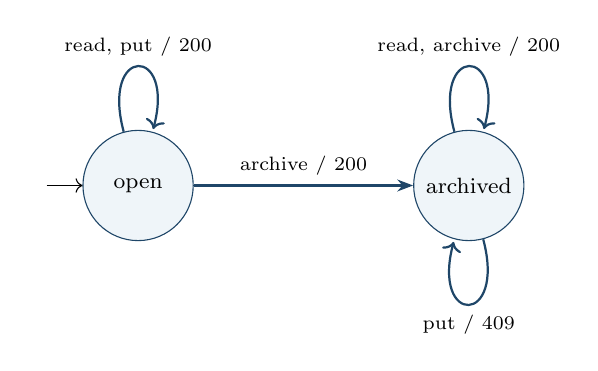
\begin{tikzpicture}[every state/.style={draw=inkblue,fill=pale,font=\footnotesize,minimum size=14mm}]
\node[state,initial,initial text={}] (o) at (0,0) {open};
\node[state] (a) at (4.2,0) {archived};
\draw[arr] (o) edge[loop above] node[above,font=\scriptsize]{read, put / 200}(o);
\draw[arr] (o)--node[above,font=\scriptsize]{archive / 200}(a);
\draw[arr] (a) edge[loop above] node[above,font=\scriptsize]{read, archive / 200}(a);
\draw[arr] (a) edge[loop below] node[below,font=\scriptsize]{put / 409}(a);
\end{tikzpicture}
\caption{Checked document policy for $h=1$ (event / status). Every usable table induces exactly this machine for all event sequences.}\label{fig:policy}
\end{figure}

A change from $h=0$ to $h=1$ changes the implementation job's signature although the interface is unchanged (the 409 clause of Section~\ref{sec:motivation}). Old pending tables cannot commit, and a current accepted table carries the trace guarantee of Fig.~\ref{fig:policy}. This guarantee comes from restricting the proposal language and trusting a small interpreter. It does not transfer to unrestricted patches that merely implement a similar interface.

\subsection{Reference Controller, Formal Model and Proofs}\label{sec:artifact}
\emph{Reference controller.} A Python implementation (about 450 lines, \texttt{src/vgc}) realizes the transitions of Table~\ref{tab:rules} for the case study. It serializes public actions with one lock. Every action copies a private candidate, installs effects there, recomputes the complete downstream structure, and installs the candidate only on success. Observations are canonical JSON containing the owner, contract, source clause, usable predecessor values and the full membership of the selected findings. Context version numbers are excluded, because agents do not see them. Request identities $(j,e,n)$ are unique within one controller lifetime. Proposal providers are deterministic or adversarial scripts; no model credentials or remote calls are involved. A separately implemented \emph{trace checker} replays recorded events and independently re-evaluates state continuity, ranked availability, exact observations, dispatch identities and counters, provenance, authority, rollback and publication snapshots.

\emph{Formal model.} \texttt{Core.tla} and \texttt{AsyncController.tla} formalize ranked prerequisites, exact observations, historical acceptance, episode counters, request history, suspension, contract and authority changes, and publication evidence in TLA$^+$~\cite{lamport1994tla,lamport2002specifying}. The value relation is abstract: a proposal is valid when it equals the observed source value. \texttt{AtomicController.tla} specifies the abstract machine $\mathcal A$.

\emph{Mechanized lemmas.} Four TLAPS~\cite{cousineau2012tlaps} modules check individual proof steps. \texttt{Budget} bounds the counter within one episode. \texttt{ControllerSafety} shows that the commit guard implies a current, authorized, valid commit. \texttt{StructuralKernelProofs} establishes coverage, unique producers and reference range under the construction hypotheses of Theorem~\ref{thm:kernel}. \texttt{DocumentPolicyProofs} establishes validator equivalence, archive absorption and the archived-\textsf{put} conflict. The full inductive invariant of Theorem~\ref{thm:safety} and the refinement mapping of Theorem~\ref{thm:refinement} are not yet mechanized (Table~\ref{tab:evidence}).

% =====================================================================
\section{Evaluation}\label{sec:evaluation}

\subsection{Research Questions}
The guarantees of Section~\ref{sec:guarantees} are proved on paper. The evaluation asks whether they hold in an executable instantiation, whether each mechanism is necessary, and what they buy in practice.
\begin{itemize}
\item[\RQ{1}] \emph{Safety and guard necessity.} Does the controller preserve its safety properties under adversarial asynchronous executions, and does removing any single mechanism break the property it is meant to protect?
\item[\RQ{2}] \emph{Locality and cost.} How much generation does exact dependency tracking avoid compared with coarser invalidation strategies, how does this scale with workspace size, and does it ever change the outcome?
\item[\RQ{3}] \emph{Behavior under change.} Does the reference implementation handle each class of workflow change exactly as the semantics prescribes?
\item[\RQ{4}] \emph{Assurance.} What do the mechanized proofs, bounded model checks and exhaustive checks establish, and what remains open?
\end{itemize}

\subsection{Experimental Setup}
\emph{Subjects.} All experiments use the case study of Section~\ref{sec:case-study}: the TLA$^+$ model for model checking, and the Python reference controller for everything else.

\emph{Why no real LLM?} The safety and locality guarantees quantify over \emph{all} proposals; for safety the proposal source is fully nondeterministic. Real model calls would add cost and nondeterminism without exercising behaviors that an adversarial script cannot produce. Our adversarial provider therefore returns valid proposals, locally valid but structurally or jointly inconsistent proposals, malformed values, and plausible answers to a \emph{different} policy question. It also delivers replies late, out of order, duplicated or never. Section~\ref{sec:threats} discusses what this choice does and does not cover.

\emph{RQ1 ablation harness.} We drive the reference controller and ten variants, each of which removes exactly one mechanism (two remove both obsolete-reply defenses, as in the formal mutants). Every variant reuses the reference code and overrides only the removed check. Each run starts with one to three documents, budget $k=2$, and executes \AblSteps{} randomly chosen actions. The actions are: dispatch; delivery in random order, possibly duplicated; timeout; source edits that flip a policy, add or delete a document; context updates, including equal-content rewrites, unselected findings and availability toggles; contract changes; owner revocation and regrant; adding or removing the reviewer; cooperative repair bursts; and publication attempts. All variants use the same \AblRuns{} seeds. An \emph{independent oracle} judges the state after every transaction. It recomputes each job's effective observation from the authoritative inputs, remembers the observation each request was dispatched against, and tracks dependency episodes itself; it never reads the controller's signatures. It checks seven properties:
P1 no value is exposed as usable whose evidence was produced for a different or unavailable observation (and no request is sent on one);
P2 no exposed value is invalid for its current observation;
P3 no value is exposed while a prerequisite is unusable;
P4 no value from a revoked owner is exposed;
P5 no ill-typed structure is installed for an active consumer;
P6 no dependency episode receives more than $k$ requests;
P7 every published snapshot is fully usable and satisfies $G$.

\emph{RQ2 cost harness.} Five strategies share validators, scheduler and guards. They differ \emph{only} in what a job's signature observes:
(i) \emph{Exact} (this paper);
(ii) \emph{No early cutoff}, where a job depends on the identity of each upstream acceptance rather than its value, as in timestamp-based build tools;
(iii) \emph{Version-keyed context}, where context readers depend on the global context version rather than on the selected content;
(iv) \emph{Whole workspace}, where every job sees all documents and the whole shared context, as in shared-message-pool frameworks;
(v) \emph{Full regeneration}, where every input change invalidates every job.
For each workspace size $N\in\{1,2,4,\ldots,\CostMaxN\}$ we generate \CostSeeds{} seeded streams of \CostChanges{} changes. Changes are source edits, selected and unselected context changes, equal-content context rewrites, and contract changes of a random stage. After each change we repair to quiescence with a correct provider. We count dispatched requests and the bytes of the observations sent, a proxy for prompt input size. Because the provider is deterministic in the observation, every strategy must accept identical values; we check this after every change.

\emph{RQ3 and RQ4.} The \Scenarios{} scenarios and their expectations are fixed in advance in \texttt{campaign.json}. Model checking uses TLC~\cite{yu1999tlc} with one worker and a 768\,MB heap. Proofs run TLAPS with its bundled Z3 4.8.9 in a pinned Linux container, in strict mode and with fingerprints erased. Python \PythonVersion{} was used throughout.

\subsection{RQ1: Safety and Necessity of Each Guard}\label{sec:rq1}
\emph{Bounded model checking.} Table~\ref{tab:tlc} reports nine baseline configurations, nine mutants and five nonvacuity witnesses. All baseline configurations satisfy the safety invariants exhaustively, with up to \TLCMaxStates{} distinct states. The frozen-input chain also satisfies eventual terminal classification under weak fairness. Seven of the nine mutants violate their targeted property within two or three actions; for example, removing both obsolete-reply defenses admits ``dispatch, edit, obsolete commit''. The two survivors each remove only one of the two obsolete-reply defenses, and the remaining defense blocks the stale commit, exactly as predicted in Section~\ref{sec:guarantees}. The witnesses confirm that acceptance, exhaustion, suspension, publication and contract change are all reachable. The safety results are therefore not vacuous.

% Generated by experiments/tse_paper.py; do not edit.
\begin{table}[!t]
\centering
\caption{Bounded TLC model checking of the protocol model. $J$: jobs; $k$: attempt cap; $m$: bound on environmental changes; \emph{Distinct}/\emph{Total}: distinct and generated states; \emph{Path}: actions in the shortest counterexample or witness. All 23 runs met their expectation (108\,s in total, one worker).}\label{tab:tlc}
\scriptsize\setlength{\tabcolsep}{2.6pt}
\begin{tabular*}{\columnwidth}{@{\extracolsep{\fill}}lrrrrrrl@{}}\toprule
Configuration & $J$ & $k$ & $m$ & Distinct & Total & Path & Result\\\midrule
\multicolumn{8}{@{}l}{\textit{Baseline protocol (safety invariants; liveness where stated)}}\\
One job & 1 & 1 & 1 & 87 & 316 & -- & Pass\\
One job & 1 & 2 & 1 & 227 & 1,061 & -- & Pass\\
Two-job chain & 2 & 1 & 1 & 292 & 1,307 & -- & Pass\\
Two-job chain, frozen & 2 & 2 & 0 & 23 & 107 & -- & Pass\\
Fan-out, frozen & 3 & 1 & 0 & 20 & 95 & -- & Pass\\
Four-stage workflow, frozen & 4 & 1 & 0 & 14 & 63 & -- & Pass\\
Observation reversion & 1 & 1 & 2 & 1,028 & 4,430 & -- & Pass\\
Reordered delivery & 2 & 1 & 1 & 475 & 2,345 & -- & Pass\\
Chain, liveness & 2 & 2 & 0 & 23 & 107 & -- & Pass\\
\midrule
\multicolumn{8}{@{}l}{\textit{Mutants (one guard removed; target property in Table~\ref{tab:boundaries})}}\\
Cancellation removed & 1 & 1 & 1 & 93 & 328 & -- & Survives\textsuperscript{a}\\
Commit recheck removed & 1 & 1 & 1 & 87 & 358 & -- & Survives\textsuperscript{a}\\
Both obsolete defences removed & 1 & 1 & 1 & 31 & 69 & 3 & Violated\\
Exhausted budget reset & 1 & 1 & 1 & 45 & 89 & 3 & Violated\\
Suspension ignored & 1 & 1 & 1 & 14 & 20 & 2 & Violated\\
Authority ignored & 1 & 1 & 1 & 32 & 98 & 3 & Violated\\
Revision check removed & 1 & 1 & 1 & 14 & 21 & 2 & Violated\\
Contract omitted & 1 & 1 & 1 & 33 & 60 & 3 & Violated\\
Selected context omitted & 1 & 1 & 1 & 32 & 57 & 3 & Violated\\
\midrule
\multicolumn{8}{@{}l}{\textit{Nonvacuity witnesses (negated reachability goal)}}\\
Acceptance & 1 & 1 & 1 & 21 & 32 & 2 & Reached\\
Budget exhaustion & 1 & 1 & 1 & 22 & 33 & 2 & Reached\\
Suspension & 1 & 1 & 1 & 6 & 7 & 1 & Reached\\
Publication (empty workflow) & 1 & 1 & 1 & 14 & 21 & 2 & Reached\\
Contract change & 1 & 1 & 1 & 5 & 6 & 1 & Reached\\
\bottomrule\end{tabular*}
\par\smallskip\raggedright\footnotesize\textsuperscript{a}Survives because the other obsolete-response defence still blocks the stale commit; see RQ1.
\end{table}


\emph{Implementation-level ablation.} The model-checking mutants use one job and one environmental change. Fig.~\ref{fig:ablation} asks the same question of the real implementation, with multiple documents, concurrent replies and adversarial proposals. Across \AblRuns{} runs, the reference controller showed \textbf{no} violation of any property (\FullViolRuns{} runs with a violation). It still published in \FullPubRuns{} runs (\FullPublications{} publications), so the absence of violations is not due to inactivity. Every non-redundant ablation was detected, each on the property it targets:
\begin{itemize}
\item removing both obsolete-reply defenses exposed stale values in \ObsoleteStalePct\% of runs, and in \ObsoleteInvalidPct\% values that were \emph{invalid} for the current input: a plausible answer to the old question is not merely outdated but wrong;
\item omitting the contract from the signature did so in \ContractStalePct\%, and omitting selected context in \ContextStalePct\%;
\item removing the upstream gate exposed values over stale prerequisites in \UpstreamPct\%;
\item ignoring authority exposed revoked owners' values in \AuthorityPct\%;
\item skipping candidate normalization installed ill-typed structure in \CandidatePct\%;
\item resetting budgets exceeded $k$ requests per episode in \BudgetPct\%;
\item dropping the global predicate published inconsistent snapshots in \GlobalPublishPct\%.
\end{itemize}
Removing \emph{one} obsolete-reply defense (cancellation or recheck) again produced no violation, which replicates the model-checking result at implementation scale. Several ablations also violate secondary properties. Stale contracts, for example, propagate into P3 and P7, because a stale value feeds its descendants and can reach publication.

% Generated by experiments/tse_paper.py; do not edit.
\begin{figure}[!t]
\centering
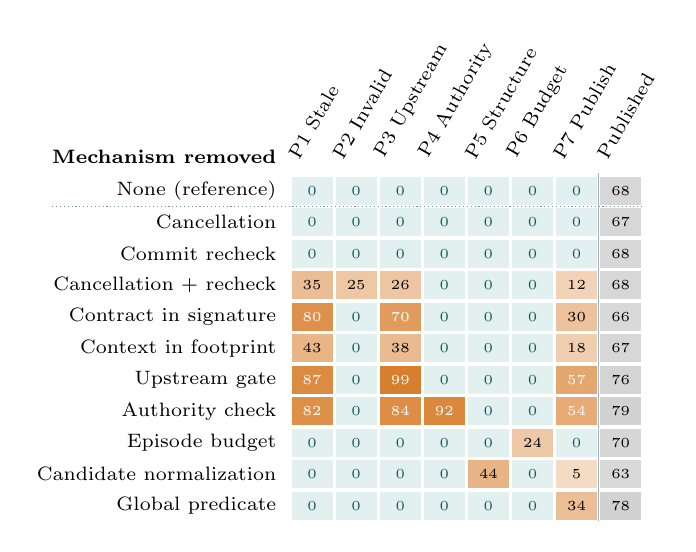
\begin{tikzpicture}
\node[rotate=60,anchor=south west,font=\scriptsize] at (-0.12,0.02) {P1 Stale};
\node[rotate=60,anchor=south west,font=\scriptsize] at (0.44,0.02) {P2 Invalid};
\node[rotate=60,anchor=south west,font=\scriptsize] at (1.00,0.02) {P3 Upstream};
\node[rotate=60,anchor=south west,font=\scriptsize] at (1.56,0.02) {P4 Authority};
\node[rotate=60,anchor=south west,font=\scriptsize] at (2.12,0.02) {P5 Structure};
\node[rotate=60,anchor=south west,font=\scriptsize] at (2.68,0.02) {P6 Budget};
\node[rotate=60,anchor=south west,font=\scriptsize] at (3.24,0.02) {P7 Publish};
\node[rotate=60,anchor=south west,font=\scriptsize] at (3.80,0.02) {Published};
\node[anchor=east,font=\scriptsize] at (-0.33,-0.20) {None (reference)};
\fill[resultteal!12!white] (-0.26,-0.38) rectangle ++(0.52,0.36);
\node[font=\tiny,text=resultteal!70!black] at (0.00,-0.20) {0};
\fill[resultteal!12!white] (0.30,-0.38) rectangle ++(0.52,0.36);
\node[font=\tiny,text=resultteal!70!black] at (0.56,-0.20) {0};
\fill[resultteal!12!white] (0.86,-0.38) rectangle ++(0.52,0.36);
\node[font=\tiny,text=resultteal!70!black] at (1.12,-0.20) {0};
\fill[resultteal!12!white] (1.42,-0.38) rectangle ++(0.52,0.36);
\node[font=\tiny,text=resultteal!70!black] at (1.68,-0.20) {0};
\fill[resultteal!12!white] (1.98,-0.38) rectangle ++(0.52,0.36);
\node[font=\tiny,text=resultteal!70!black] at (2.24,-0.20) {0};
\fill[resultteal!12!white] (2.54,-0.38) rectangle ++(0.52,0.36);
\node[font=\tiny,text=resultteal!70!black] at (2.80,-0.20) {0};
\fill[resultteal!12!white] (3.10,-0.38) rectangle ++(0.52,0.36);
\node[font=\tiny,text=resultteal!70!black] at (3.36,-0.20) {0};
\fill[gray!31!white] (3.66,-0.38) rectangle ++(0.52,0.36);
\node[font=\tiny,text=black] at (3.92,-0.20) {68};
\draw[inkblue!60,densely dotted] (-3.3,-0.40) -- (4.20,-0.40);
\node[anchor=east,font=\scriptsize] at (-0.33,-0.60) {Cancellation};
\fill[resultteal!12!white] (-0.26,-0.78) rectangle ++(0.52,0.36);
\node[font=\tiny,text=resultteal!70!black] at (0.00,-0.60) {0};
\fill[resultteal!12!white] (0.30,-0.78) rectangle ++(0.52,0.36);
\node[font=\tiny,text=resultteal!70!black] at (0.56,-0.60) {0};
\fill[resultteal!12!white] (0.86,-0.78) rectangle ++(0.52,0.36);
\node[font=\tiny,text=resultteal!70!black] at (1.12,-0.60) {0};
\fill[resultteal!12!white] (1.42,-0.78) rectangle ++(0.52,0.36);
\node[font=\tiny,text=resultteal!70!black] at (1.68,-0.60) {0};
\fill[resultteal!12!white] (1.98,-0.78) rectangle ++(0.52,0.36);
\node[font=\tiny,text=resultteal!70!black] at (2.24,-0.60) {0};
\fill[resultteal!12!white] (2.54,-0.78) rectangle ++(0.52,0.36);
\node[font=\tiny,text=resultteal!70!black] at (2.80,-0.60) {0};
\fill[resultteal!12!white] (3.10,-0.78) rectangle ++(0.52,0.36);
\node[font=\tiny,text=resultteal!70!black] at (3.36,-0.60) {0};
\fill[gray!31!white] (3.66,-0.78) rectangle ++(0.52,0.36);
\node[font=\tiny,text=black] at (3.92,-0.60) {67};
\node[anchor=east,font=\scriptsize] at (-0.33,-1.00) {Commit recheck};
\fill[resultteal!12!white] (-0.26,-1.18) rectangle ++(0.52,0.36);
\node[font=\tiny,text=resultteal!70!black] at (0.00,-1.00) {0};
\fill[resultteal!12!white] (0.30,-1.18) rectangle ++(0.52,0.36);
\node[font=\tiny,text=resultteal!70!black] at (0.56,-1.00) {0};
\fill[resultteal!12!white] (0.86,-1.18) rectangle ++(0.52,0.36);
\node[font=\tiny,text=resultteal!70!black] at (1.12,-1.00) {0};
\fill[resultteal!12!white] (1.42,-1.18) rectangle ++(0.52,0.36);
\node[font=\tiny,text=resultteal!70!black] at (1.68,-1.00) {0};
\fill[resultteal!12!white] (1.98,-1.18) rectangle ++(0.52,0.36);
\node[font=\tiny,text=resultteal!70!black] at (2.24,-1.00) {0};
\fill[resultteal!12!white] (2.54,-1.18) rectangle ++(0.52,0.36);
\node[font=\tiny,text=resultteal!70!black] at (2.80,-1.00) {0};
\fill[resultteal!12!white] (3.10,-1.18) rectangle ++(0.52,0.36);
\node[font=\tiny,text=resultteal!70!black] at (3.36,-1.00) {0};
\fill[gray!31!white] (3.66,-1.18) rectangle ++(0.52,0.36);
\node[font=\tiny,text=black] at (3.92,-1.00) {68};
\node[anchor=east,font=\scriptsize] at (-0.33,-1.40) {Cancellation + recheck};
\fill[resultamber!51!white] (-0.26,-1.58) rectangle ++(0.52,0.36);
\node[font=\tiny,text=black] at (0.00,-1.40) {35};
\fill[resultamber!43!white] (0.30,-1.58) rectangle ++(0.52,0.36);
\node[font=\tiny,text=black] at (0.56,-1.40) {25};
\fill[resultamber!44!white] (0.86,-1.58) rectangle ++(0.52,0.36);
\node[font=\tiny,text=black] at (1.12,-1.40) {26};
\fill[resultteal!12!white] (1.42,-1.58) rectangle ++(0.52,0.36);
\node[font=\tiny,text=resultteal!70!black] at (1.68,-1.40) {0};
\fill[resultteal!12!white] (1.98,-1.58) rectangle ++(0.52,0.36);
\node[font=\tiny,text=resultteal!70!black] at (2.24,-1.40) {0};
\fill[resultteal!12!white] (2.54,-1.58) rectangle ++(0.52,0.36);
\node[font=\tiny,text=resultteal!70!black] at (2.80,-1.40) {0};
\fill[resultamber!34!white] (3.10,-1.58) rectangle ++(0.52,0.36);
\node[font=\tiny,text=black] at (3.36,-1.40) {12};
\fill[gray!31!white] (3.66,-1.58) rectangle ++(0.52,0.36);
\node[font=\tiny,text=black] at (3.92,-1.40) {68};
\node[anchor=east,font=\scriptsize] at (-0.33,-1.80) {Contract in signature};
\fill[resultamber!85!white] (-0.26,-1.98) rectangle ++(0.52,0.36);
\node[font=\tiny,text=white] at (0.00,-1.80) {80};
\fill[resultteal!12!white] (0.30,-1.98) rectangle ++(0.52,0.36);
\node[font=\tiny,text=resultteal!70!black] at (0.56,-1.80) {0};
\fill[resultamber!77!white] (0.86,-1.98) rectangle ++(0.52,0.36);
\node[font=\tiny,text=white] at (1.12,-1.80) {70};
\fill[resultteal!12!white] (1.42,-1.98) rectangle ++(0.52,0.36);
\node[font=\tiny,text=resultteal!70!black] at (1.68,-1.80) {0};
\fill[resultteal!12!white] (1.98,-1.98) rectangle ++(0.52,0.36);
\node[font=\tiny,text=resultteal!70!black] at (2.24,-1.80) {0};
\fill[resultteal!12!white] (2.54,-1.98) rectangle ++(0.52,0.36);
\node[font=\tiny,text=resultteal!70!black] at (2.80,-1.80) {0};
\fill[resultamber!47!white] (3.10,-1.98) rectangle ++(0.52,0.36);
\node[font=\tiny,text=black] at (3.36,-1.80) {30};
\fill[gray!30!white] (3.66,-1.98) rectangle ++(0.52,0.36);
\node[font=\tiny,text=black] at (3.92,-1.80) {66};
\node[anchor=east,font=\scriptsize] at (-0.33,-2.20) {Context in footprint};
\fill[resultamber!57!white] (-0.26,-2.38) rectangle ++(0.52,0.36);
\node[font=\tiny,text=black] at (0.00,-2.20) {43};
\fill[resultteal!12!white] (0.30,-2.38) rectangle ++(0.52,0.36);
\node[font=\tiny,text=resultteal!70!black] at (0.56,-2.20) {0};
\fill[resultamber!53!white] (0.86,-2.38) rectangle ++(0.52,0.36);
\node[font=\tiny,text=black] at (1.12,-2.20) {38};
\fill[resultteal!12!white] (1.42,-2.38) rectangle ++(0.52,0.36);
\node[font=\tiny,text=resultteal!70!black] at (1.68,-2.20) {0};
\fill[resultteal!12!white] (1.98,-2.38) rectangle ++(0.52,0.36);
\node[font=\tiny,text=resultteal!70!black] at (2.24,-2.20) {0};
\fill[resultteal!12!white] (2.54,-2.38) rectangle ++(0.52,0.36);
\node[font=\tiny,text=resultteal!70!black] at (2.80,-2.20) {0};
\fill[resultamber!38!white] (3.10,-2.38) rectangle ++(0.52,0.36);
\node[font=\tiny,text=black] at (3.36,-2.20) {18};
\fill[gray!31!white] (3.66,-2.38) rectangle ++(0.52,0.36);
\node[font=\tiny,text=black] at (3.92,-2.20) {67};
\node[anchor=east,font=\scriptsize] at (-0.33,-2.60) {Upstream gate};
\fill[resultamber!90!white] (-0.26,-2.78) rectangle ++(0.52,0.36);
\node[font=\tiny,text=white] at (0.00,-2.60) {87};
\fill[resultteal!12!white] (0.30,-2.78) rectangle ++(0.52,0.36);
\node[font=\tiny,text=resultteal!70!black] at (0.56,-2.60) {0};
\fill[resultamber!99!white] (0.86,-2.78) rectangle ++(0.52,0.36);
\node[font=\tiny,text=white] at (1.12,-2.60) {99};
\fill[resultteal!12!white] (1.42,-2.78) rectangle ++(0.52,0.36);
\node[font=\tiny,text=resultteal!70!black] at (1.68,-2.60) {0};
\fill[resultteal!12!white] (1.98,-2.78) rectangle ++(0.52,0.36);
\node[font=\tiny,text=resultteal!70!black] at (2.24,-2.60) {0};
\fill[resultteal!12!white] (2.54,-2.78) rectangle ++(0.52,0.36);
\node[font=\tiny,text=resultteal!70!black] at (2.80,-2.60) {0};
\fill[resultamber!68!white] (3.10,-2.78) rectangle ++(0.52,0.36);
\node[font=\tiny,text=white] at (3.36,-2.60) {57};
\fill[gray!34!white] (3.66,-2.78) rectangle ++(0.52,0.36);
\node[font=\tiny,text=black] at (3.92,-2.60) {76};
\node[anchor=east,font=\scriptsize] at (-0.33,-3.00) {Authority check};
\fill[resultamber!86!white] (-0.26,-3.18) rectangle ++(0.52,0.36);
\node[font=\tiny,text=white] at (0.00,-3.00) {82};
\fill[resultteal!12!white] (0.30,-3.18) rectangle ++(0.52,0.36);
\node[font=\tiny,text=resultteal!70!black] at (0.56,-3.00) {0};
\fill[resultamber!88!white] (0.86,-3.18) rectangle ++(0.52,0.36);
\node[font=\tiny,text=white] at (1.12,-3.00) {84};
\fill[resultamber!93!white] (1.42,-3.18) rectangle ++(0.52,0.36);
\node[font=\tiny,text=white] at (1.68,-3.00) {92};
\fill[resultteal!12!white] (1.98,-3.18) rectangle ++(0.52,0.36);
\node[font=\tiny,text=resultteal!70!black] at (2.24,-3.00) {0};
\fill[resultteal!12!white] (2.54,-3.18) rectangle ++(0.52,0.36);
\node[font=\tiny,text=resultteal!70!black] at (2.80,-3.00) {0};
\fill[resultamber!65!white] (3.10,-3.18) rectangle ++(0.52,0.36);
\node[font=\tiny,text=white] at (3.36,-3.00) {54};
\fill[gray!35!white] (3.66,-3.18) rectangle ++(0.52,0.36);
\node[font=\tiny,text=black] at (3.92,-3.00) {79};
\node[anchor=east,font=\scriptsize] at (-0.33,-3.40) {Episode budget};
\fill[resultteal!12!white] (-0.26,-3.58) rectangle ++(0.52,0.36);
\node[font=\tiny,text=resultteal!70!black] at (0.00,-3.40) {0};
\fill[resultteal!12!white] (0.30,-3.58) rectangle ++(0.52,0.36);
\node[font=\tiny,text=resultteal!70!black] at (0.56,-3.40) {0};
\fill[resultteal!12!white] (0.86,-3.58) rectangle ++(0.52,0.36);
\node[font=\tiny,text=resultteal!70!black] at (1.12,-3.40) {0};
\fill[resultteal!12!white] (1.42,-3.58) rectangle ++(0.52,0.36);
\node[font=\tiny,text=resultteal!70!black] at (1.68,-3.40) {0};
\fill[resultteal!12!white] (1.98,-3.58) rectangle ++(0.52,0.36);
\node[font=\tiny,text=resultteal!70!black] at (2.24,-3.40) {0};
\fill[resultamber!42!white] (2.54,-3.58) rectangle ++(0.52,0.36);
\node[font=\tiny,text=black] at (2.80,-3.40) {24};
\fill[resultteal!12!white] (3.10,-3.58) rectangle ++(0.52,0.36);
\node[font=\tiny,text=resultteal!70!black] at (3.36,-3.40) {0};
\fill[gray!32!white] (3.66,-3.58) rectangle ++(0.52,0.36);
\node[font=\tiny,text=black] at (3.92,-3.40) {70};
\node[anchor=east,font=\scriptsize] at (-0.33,-3.80) {Candidate normalization};
\fill[resultteal!12!white] (-0.26,-3.98) rectangle ++(0.52,0.36);
\node[font=\tiny,text=resultteal!70!black] at (0.00,-3.80) {0};
\fill[resultteal!12!white] (0.30,-3.98) rectangle ++(0.52,0.36);
\node[font=\tiny,text=resultteal!70!black] at (0.56,-3.80) {0};
\fill[resultteal!12!white] (0.86,-3.98) rectangle ++(0.52,0.36);
\node[font=\tiny,text=resultteal!70!black] at (1.12,-3.80) {0};
\fill[resultteal!12!white] (1.42,-3.98) rectangle ++(0.52,0.36);
\node[font=\tiny,text=resultteal!70!black] at (1.68,-3.80) {0};
\fill[resultamber!58!white] (1.98,-3.98) rectangle ++(0.52,0.36);
\node[font=\tiny,text=black] at (2.24,-3.80) {44};
\fill[resultteal!12!white] (2.54,-3.98) rectangle ++(0.52,0.36);
\node[font=\tiny,text=resultteal!70!black] at (2.80,-3.80) {0};
\fill[resultamber!28!white] (3.10,-3.98) rectangle ++(0.52,0.36);
\node[font=\tiny,text=black] at (3.36,-3.80) {5};
\fill[gray!30!white] (3.66,-3.98) rectangle ++(0.52,0.36);
\node[font=\tiny,text=black] at (3.92,-3.80) {63};
\node[anchor=east,font=\scriptsize] at (-0.33,-4.20) {Global predicate};
\fill[resultteal!12!white] (-0.26,-4.38) rectangle ++(0.52,0.36);
\node[font=\tiny,text=resultteal!70!black] at (0.00,-4.20) {0};
\fill[resultteal!12!white] (0.30,-4.38) rectangle ++(0.52,0.36);
\node[font=\tiny,text=resultteal!70!black] at (0.56,-4.20) {0};
\fill[resultteal!12!white] (0.86,-4.38) rectangle ++(0.52,0.36);
\node[font=\tiny,text=resultteal!70!black] at (1.12,-4.20) {0};
\fill[resultteal!12!white] (1.42,-4.38) rectangle ++(0.52,0.36);
\node[font=\tiny,text=resultteal!70!black] at (1.68,-4.20) {0};
\fill[resultteal!12!white] (1.98,-4.38) rectangle ++(0.52,0.36);
\node[font=\tiny,text=resultteal!70!black] at (2.24,-4.20) {0};
\fill[resultteal!12!white] (2.54,-4.38) rectangle ++(0.52,0.36);
\node[font=\tiny,text=resultteal!70!black] at (2.80,-4.20) {0};
\fill[resultamber!50!white] (3.10,-4.38) rectangle ++(0.52,0.36);
\node[font=\tiny,text=black] at (3.36,-4.20) {34};
\fill[gray!35!white] (3.66,-4.38) rectangle ++(0.52,0.36);
\node[font=\tiny,text=black] at (3.92,-4.20) {78};
\draw[inkblue!40] (3.64,0.02) -- (3.64,-4.40);
\node[anchor=south east,font=\scriptsize\bfseries] at (-0.33,0.02) {Mechanism removed};
\end{tikzpicture}
\caption{RQ1: implementation-level guard ablation under 300 seeded adversarial executions per variant (120 steps each). Cells give the percentage of runs in which the independent oracle observed at least one violation of property P1--P7 (Section~\ref{sec:rq1}); the last column gives the percentage of runs that published at least once. The reference controller (top row) shows no violation. Removing either obsolete-response defence alone is masked by the other.}\label{fig:ablation}
\end{figure}


\emph{A defect found by the campaign.} The randomized campaign also exposed a robustness defect in the original reference implementation. \texttt{edit\_source} and \texttt{reconfigure} record a rejection when candidate normalization fails, but \texttt{update\_context} let the exception escape. The path is as follows. Context becomes unavailable, so the implementation stage is suspended. An integer-identifier architecture is then committed, which is admissible because no active consumer exists. Re-enabling the context fails normalization. With the same seeds, the unfixed controller raised this exception in \PreFixApiRuns{} of \PreFixRuns{} reference runs (\PreFixApiExceptions{} exceptions in total). The state remained atomic, because the failure occurred on the private candidate, and no safety property was violated (\PreFixViolRuns{} runs with a violation), but the API broke its contract. We fixed the defect (the action now records the rejection) and added a regression test. The underlying semantic subtlety is now listed as a limitation (Section~\ref{sec:limitations}). We also found that the original candidate constructor instantiated the base class, which silently bypassed overridden checks in subclasses; it now preserves the subclass type. The numbers above are from the fixed implementation.

\textbf{Answer to RQ1.} No safety violation was observed in \TLCBaselines{} exhaustive model-checking configurations or in \AblRuns{} randomized adversarial executions of the reference controller. Each of the \AblDetected{} ablations that remove a non-redundant mechanism violated its targeted property, both in the model (where a corresponding mutant exists) and in the implementation. The cancellation and recheck defenses are individually redundant but jointly necessary.

\subsection{RQ2: Locality and Cost}\label{sec:rq2}
Fig.~\ref{fig:cost} plots generation requests and observation bytes per change against workspace size, and Table~\ref{tab:cost} breaks requests down by change type for $N=\CostMaxN$. With exact signatures, cost grows only with the number of jobs a change actually affects. A source edit regenerates that document's four jobs. A selected-context change regenerates the two jobs that read the finding. Unselected changes and equal-content rewrites regenerate nothing. Only contract changes touch every job of the changed stage, because every such job's contract changed. Full regeneration and the whole-workspace footprint instead scale linearly with $N$. At $N=\CostMaxN$, exact signatures needed \ExactReqMaxN{} requests per change on average, versus \FullReqMaxN{} for full regeneration: a \RatioFull$\times$ reduction. The reduction is \RatioWorkspace$\times$ against the whole-workspace footprint, \RatioVersion$\times$ against version-keyed context, and \RatioCutoff$\times$ against the strategy without early cutoff.

The savings in transmitted observation size are larger still, because a whole-workspace observation also grows with $N$. Per change, the whole-workspace strategy sent \BytesRatioWorkspace$\times$ the bytes of the exact strategy, and full regeneration \BytesRatioFull$\times$. Exact observations are small and their size is independent of $N$. In every run, all five strategies accepted identical values after every change (outcome equivalence: \CostEquivalent{} runs). Coarser footprints are thus sound but wasteful, and the savings never come at the price of a different result.

% Generated by experiments/tse_paper.py; do not edit.
\begin{figure*}[!t]
\centering
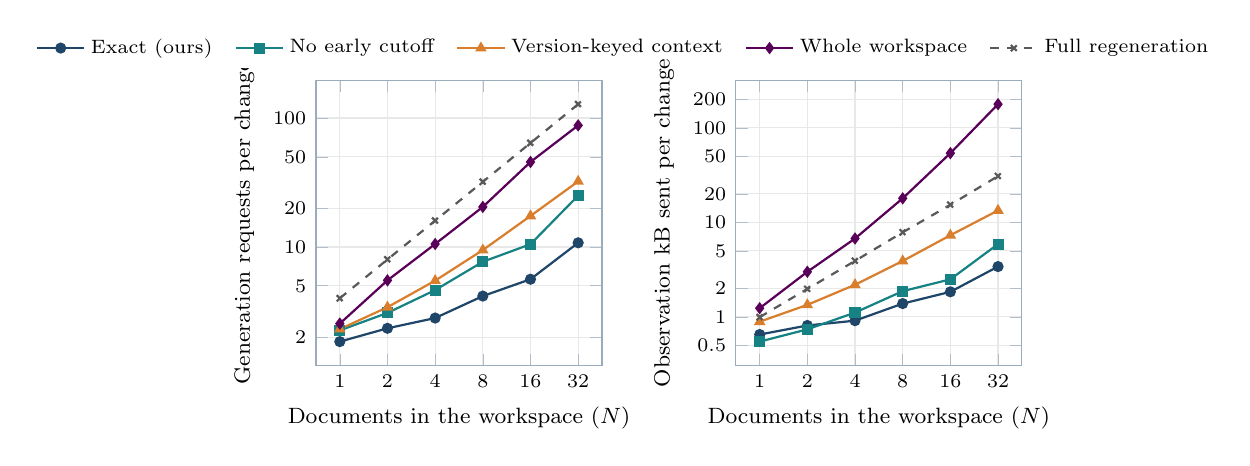
\begin{tikzpicture}
\begin{groupplot}[group style={group size=2 by 1,horizontal sep=1.7cm},vgcplot,width=.43\textwidth,height=5.2cm,
  xmode=log,log basis x=2,ymode=log,xtick={1,2,4,8,16,32},xticklabels={1,2,4,8,16,32},log ticks with fixed point,
  ytick={0.1,0.2,0.5,1,2,5,10,20,50,100,200,500,1000,2000},xlabel={Documents in the workspace ($N$)},
  legend style={at={(1.08,1.04)},anchor=south,legend columns=5,draw=none,/tikz/every even column/.append style={column sep=6pt}}]
\nextgroupplot[ylabel={Generation requests per change}]
\addplot[inkblue,mark=*,thick,mark size=1.6pt] coordinates {(1,1.845) (2,2.34) (4,2.81) (8,4.16) (16,5.62) (32,10.77)};
\addplot[resultteal,mark=square*,thick,mark size=1.6pt] coordinates {(1,2.255) (2,3.08) (4,4.63) (8,7.68) (16,10.5) (32,25.01)};
\addplot[resultamber,mark=triangle*,thick,mark size=1.6pt] coordinates {(1,2.305) (2,3.41) (4,5.48) (8,9.46) (16,17.4) (32,32.24)};
\addplot[violet!70!black,mark=diamond*,thick,mark size=1.6pt] coordinates {(1,2.545) (2,5.51) (4,10.54) (8,20.44) (16,45.6) (32,87.68)};
\addplot[gray!70!black,mark=x,dashed,thick,mark size=1.6pt] coordinates {(1,4) (2,8) (4,16) (8,32) (16,64) (32,128)};
\legend{Exact (ours),No early cutoff,Version-keyed context,Whole workspace,Full regeneration}
\nextgroupplot[ylabel={Observation kB sent per change}]
\addplot[inkblue,mark=*,thick,mark size=1.6pt] coordinates {(1,0.6504) (2,0.8106) (4,0.9113) (8,1.382) (16,1.84) (32,3.404)};
\addplot[resultteal,mark=square*,thick,mark size=1.6pt] coordinates {(1,0.5473) (2,0.7381) (4,1.11) (8,1.87) (16,2.494) (32,5.888)};
\addplot[resultamber,mark=triangle*,thick,mark size=1.6pt] coordinates {(1,0.8893) (2,1.34) (4,2.186) (8,3.899) (16,7.299) (32,13.35)};
\addplot[violet!70!black,mark=diamond*,thick,mark size=1.6pt] coordinates {(1,1.235) (2,2.998) (4,6.741) (8,17.93) (16,53.89) (32,177.7)};
\addplot[gray!70!black,mark=x,dashed,thick,mark size=1.6pt] coordinates {(1,0.9932) (2,1.974) (4,3.907) (8,7.842) (16,15.33) (32,30.82)};
\end{groupplot}
\end{tikzpicture}
\caption{RQ2: generation work per input change as the workspace grows (log--log; mean over 5 seeds $\times$ 40 random changes per size). All strategies share validators, scheduler and guards and differ only in what a job's signature observes; they accepted identical values in every run. Left: dispatched requests. Right: total size of the observations sent to workers, a proxy for prompt input tokens.}\label{fig:cost}
\end{figure*}

% Generated by experiments/tse_paper.py; do not edit.
\begin{table}[!t]
\centering
\caption{RQ2: mean generation requests per change by change type for $N=32$ documents. Exact signatures make the cost of source and context changes independent of $N$; contract changes necessarily touch every job of the changed stage.}\label{tab:cost}
\scriptsize\setlength{\tabcolsep}{2pt}
\begin{tabular*}{\columnwidth}{@{\extracolsep{\fill}}lrrrrr@{}}\toprule
Change type & \rotatebox{70}{Exact (ours)} & \rotatebox{70}{No early cutoff} & \rotatebox{70}{Version-keyed context} & \rotatebox{70}{Whole workspace} & \rotatebox{70}{Full regeneration}\\\midrule
Source clause edit & 4.0 & 4.0 & 4.0 & 128.0 & 128.0\\
Selected finding changed & 2.0 & 2.0 & 64.0 & 128.0 & 128.0\\
Unselected finding changed & 0.0 & 0.0 & 64.0 & 128.0 & 128.0\\
Equal content, new version & 0.0 & 0.0 & 64.0 & 0.0 & 128.0\\
Contract change & 32.0 & 82.9 & 32.0 & 32.0 & 128.0\\
\midrule All changes & 10.8 & 25.0 & 32.2 & 87.7 & 128.0\\
Bytes per request & 316 & 235 & 414 & 2,027 & 241\\
\bottomrule\end{tabular*}
\end{table}


The scenario campaign confirms the mechanism on individual interventions. A repair pass with no relevant change (S02), an unselected context update (S08) and a new context version with equal selected content (S10) caused no request at all. An architecture contract change repaired to an equal output caused exactly one request, because early cutoff restored the descendants from cache (S16). A tightened clause propagated to all four views, because their observations changed despite the unchanged interface (S17).

\textbf{Answer to RQ2.} Exact dependency signatures make the generation cost of source and context changes independent of workspace size. At $N=\CostMaxN$ they reduce requests per change by \RatioFull$\times$ relative to full regeneration and by \RatioCutoff--\RatioWorkspace$\times$ relative to plausible coarser strategies, with identical outcomes in all runs. These counts are structural: they measure avoided generation calls, not LLM latency or price.

\subsection{RQ3: Behavior Under Change}\label{sec:rq3}
Table~\ref{tab:scenarios} groups the \Scenarios{} scenarios by the class of change they exercise and maps each class to the guarantee it tests. All \ScenarioPasses{} scenarios met their predefined expectations. Many expectations are refusals: a discarded late reply (S11--S13), an exhausted episode that earns no new budget (S14), a blocked descendant (S15), a joint conflict (S18), a rolled-back candidate (S19), a reviewer whose addition blocks publication until it has assessed every operation (S20), and a rejected publication based on a stale check (S25). Three scenarios published successfully with nonempty generated work (S01, S20 after repair, and S26). The trace checker admitted all \Scenarios{} recorded traces and rejected all \Corruptions{} deliberately corrupted ones. The corruptions include acceptance events that hide a source, context or contract change behind a valid value.

% Generated by experiments/tse_paper.py; do not edit.
\begin{table*}[!t]
\centering
\caption{The 28 scripted change scenarios, grouped by the class of change they exercise. Event counts come from the recorded traces: D dispatched requests, A accepted replies, R current rejections or timeouts, X obsolete or duplicate replies discarded, E committed edits/reconfigurations, B refused edits or publications, P publications. A scenario passes when its independently written expectation holds; for several scenarios the expected outcome is a refusal.}\label{tab:scenarios}
\footnotesize\setlength{\tabcolsep}{4pt}
\begin{tabular*}{\textwidth}{@{\extracolsep{\fill}}llcrrrrrrrc@{}}\toprule
Change class & Scenarios (S\#) & Guarantee exercised & D & A & R & X & E & B & P & Pass\\\midrule
Initial completion and no-op repair & 01, 02 & Thm.~\ref{thm:safety}, \ref{thm:local} & 8 & 8 & 0 & 0 & 0 & 0 & 1 & 2/2\\
Source edits, additions, deletions & 03, 04, 05, 06, 17 & Thm.~\ref{thm:kernel}, \ref{thm:local} & 28 & 28 & 0 & 0 & 6 & 0 & 0 & 5/5\\
Shared-context changes and writers & 07, 08, 09, 10, 24 & Thm.~\ref{thm:local}, Prop.~\ref{prop:isolation} & 18 & 18 & 0 & 0 & 6 & 1 & 0 & 5/5\\
Obsolete, late, duplicate replies & 11, 12, 13 & Thm.~\ref{thm:safety}(iv), \ref{thm:refinement} & 3 & 0 & 1 & 4 & 3 & 0 & 0 & 3/3\\
Budget exhaustion and blocking & 14, 15 & Thm.~\ref{thm:cost}, \ref{thm:termination} & 4 & 0 & 4 & 0 & 2 & 4 & 0 & 2/2\\
Contract change and early cutoff & 16, 23 & Thm.~\ref{thm:local}, \ref{thm:reconfig} & 10 & 9 & 0 & 1 & 3 & 0 & 0 & 2/2\\
Joint conflict, rollback, stale check & 18, 19, 25 & Thm.~\ref{thm:safety}(i),(v) & 14 & 13 & 1 & 0 & 3 & 2 & 0 & 3/3\\
Reviewer and authority changes & 20, 21, 22 & Thm.~\ref{thm:reconfig} & 10 & 9 & 0 & 1 & 4 & 3 & 1 & 3/3\\
Untrusted ingress, observer loss & 26, 27 & Prop.~\ref{prop:observation} & 4 & 4 & 0 & 0 & 0 & 2 & 1 & 2/2\\
Finite policy language (exhaustive) & 28 & Thm.~\ref{thm:table} & 0 & 0 & 0 & 0 & 0 & 0 & 0 & 1/1\\
\midrule\textbf{All scenarios} & 01--28 & & 99 & 89 & 6 & 6 & 27 & 12 & 3 & 28/28\\
\bottomrule\end{tabular*}
\end{table*}


Two observations deserve emphasis. First, \emph{reversion does not restore authority}: in S12 the clause changes and then reverts, so the observation bytes return to their original value, but the cancelled request still cannot commit, because the reversion started a new episode. Signatures alone therefore do not give idempotent delivery; request identities are needed as well. Second, \emph{equal content is not a change}: in S10 the shared context is republished at a new version with the same selected findings, and no job is invalidated, because agents never see version numbers (Section~\ref{sec:semantics}).

\textbf{Answer to RQ3.} The reference implementation behaved as the semantics prescribes for all ten change classes, including the refusal cases, and an independent checker confirmed every recorded trace.

\subsection{RQ4: Assurance and Remaining Obligations}\label{sec:rq4}
Table~\ref{tab:assurance} summarizes the mechanized and exhaustive evidence. The four TLAPS modules discharge \ProvedObligations{} obligations. The preserved first development run failed three obligations in two modules: proof steps that lacked explicit references to construction and type assumptions. No assumption equivalent to the safety conclusion was added to repair them. For the restricted policy language, exhaustive enumeration of all \PolicyTables{} typed tables (both policies) confirmed that the validator accepts exactly one table per policy. All \EventWords{} event words of length at most six obey the trace properties of Theorem~\ref{thm:table}. Two clean re-runs from packaged archives reproduced every reported outcome; both predate the defect fix of Section~\ref{sec:rq1}, after which the scenario, conformance and test stages were re-run.

% Generated by experiments/tse_paper.py; do not edit.
\begin{table}[!t]
\centering
\caption{Assurance evidence. For proofs, \emph{Final} counts proved/total obligations in the clean run and \emph{First trial} the preserved failed development run. Executable counts are exhaustive where stated; the other checks cover the recorded executions only.}\label{tab:assurance}
\scriptsize\setlength{\tabcolsep}{2.5pt}
\begin{tabular*}{\columnwidth}{@{\extracolsep{\fill}}>{\raggedright\arraybackslash}p{24mm}>{\raggedright\arraybackslash}p{28mm}rl@{}}\toprule
Artifact & Scope & Final & First trial\\\midrule
\multicolumn{4}{@{}l}{\textit{Mechanized TLAPS lemmas (strict mode, fingerprints erased)}}\\
{\ttfamily Budget} & Counter bound for one episode & 8/8 & 1 of 7 failed\\
{\ttfamily ControllerSafety} & Commit guard implies current, authorized, valid commit & 2/2 & 0 of 2 failed\\
{\ttfamily StructuralKernel} & Kernel coverage, unique producers, reference range & 9/9 & 2 of 6 failed\\
{\ttfamily DocumentPolicy} & Validator equivalence; archived-put conflict & 6/6 & 0 of 6 failed\\
\midrule\multicolumn{4}{@{}l}{\textit{Executable checks}}\\
Policy tables & All typed six-row tables, both policies & 8,192 & exhaustive\\
Event words & All words of length $\le 6$, strict table & 1,093 & exhaustive\\
Trace checker & Recorded scenario traces admitted & 28/28 & --\\
Trace checker & Deliberately corrupted traces rejected & 9/9 & --\\
Regression tests & Transaction-boundary unit tests & 13/13 & --\\
Reproduction & Clean re-runs of packaged archives matched (pre-fix snapshots) & 2/2 & --\\
\bottomrule\end{tabular*}
\end{table}


The evidence is deliberately uneven, and Table~\ref{tab:evidence} makes this explicit. Lemmas used inside the safety and budget proofs are mechanized, but the full inductive invariant, the history-counting argument across episodes, and the refinement mapping to \texttt{AtomicController.tla} are proved only on paper. Bounded model checking covers instances with at most four jobs. The implementation-level ablation (RQ1) and the scenario campaign (RQ3) cover larger, concurrent executions of the reference controller, but by testing rather than proof.

\textbf{Answer to RQ4.} The scoped lemmas, bounded model checks and exhaustive checks corroborate the paper proofs at every level we could mechanize. The central parameterized invariant and the refinement mapping remain open mechanization targets.

\subsection{Implications for Builders of Agent Frameworks}\label{sec:implications}
The results suggest concrete design rules for orchestrators of LLM agents, such as graph-based or conversation-based frameworks.
\begin{enumerate}
\item \emph{Key every generated artifact by its exact observation, including the prompt and validator version.} RQ1 shows that omitting the contract or the selected context from the key exposes stale artifacts in a large fraction of runs. RQ2 shows that keying by content rather than by version or timestamp avoids most regeneration.
\item \emph{Give every request an identity, and recheck currentness at commit time.} Either defense alone prevented stale commits in RQ1, but they serve different purposes, so keep both. The commit-time recheck is what makes acceptance safe. Cancellation additionally frees the job: without it, an obsolete request stays pending and blocks re-dispatch until its reply arrives or times out.
\item \emph{Separate ``accepted'' from ``usable'', and gate consumers on usability.} Removing the upstream gate was the most frequently detected ablation.
\item \emph{Make completion a global predicate, recomputed after every change of team or rules.} Locally valid outputs that disagree reach publication otherwise.
\item \emph{Budget per dependency episode, not per scheduler pass.} Per-pass budgets let a failing request be retried indefinitely.
\end{enumerate}
The interesting fact here is: \textit{none of these rules depends on how good the underlying model is.}

% =====================================================================
\section{Threats to Validity}\label{sec:threats}
\emph{Construct validity.} Our safety properties P1--P7 operationalize Theorem~\ref{thm:safety} and Theorem~\ref{thm:cost}. The oracle recomputes observations from the specification, but it shares the case study's definitions of footprint and validator with the controller. A shared misunderstanding of those definitions would go undetected. Observation bytes are only a proxy for prompt tokens, and request counts measure avoided calls, not latency or monetary cost.

\emph{Internal validity.} Each ablation reuses the reference code and overrides only the removed check, which limits confounding. We found and fixed one harness problem during development, a base-class candidate constructor that silently bypassed overrides; all reported numbers come from the corrected harness. Scenario expectations were written by the author before execution. They are fixed in the repository, but they are not independent of the designer's understanding of the semantics. The trace checker trusts recorded events and cannot detect an omitted final suffix.

\emph{External validity.} We used scripted and adversarial providers instead of real LLMs. This is sound for safety, because the semantics quantifies over all proposals, and for structural cost, because request counts do not depend on answer quality. It does not tell us how often real models produce invalid or conflicting proposals, or how much wall-clock time the savings represent. The case study is small (four or five views per document, a six-row behavioral language), and bounded model checking covers at most four jobs. Larger artifact languages, such as full source files with test-suite validators, make footprint adequacy and validator soundness harder to establish (Example~\ref{ex:limits}).

\emph{Conclusion validity.} The runs are deterministic functions of their seeds and are not independent samples of a deployment population. We therefore report counts and proportions, not significance tests. All seeds, configurations and source hashes are recorded with the results.

% =====================================================================
\section{Related Work}\label{sec:related}
\emph{LLM-based multi-agent software engineering.} MetaGPT~\cite{metagpt} encodes standard operating procedures as role prompts and structured hand-offs. ChatDev~\cite{chatdev} organizes agents into a chat chain, and AutoGen~\cite{autogen} provides programmable multi-agent conversation. SWE-agent~\cite{sweagent} studies agent--computer interfaces for repository-level repair, evaluated on SWE-bench~\cite{swebench}. Surveys map this landscape~\cite{hou2024llm4se,he2025mas,wang2024agents}. Cemri et al.~\cite{cemri2025mast} analyze failures of multi-agent LLM systems and report specification issues, inter-agent misalignment and task-verification failures as major categories. These works orchestrate agents by conversation or fixed pipelines. Our work is complementary: it specifies when an agent's output may be accepted, reused and released, and it proves properties that hold for any agent behavior. The rules of Section~\ref{sec:implications} could be adopted by these frameworks.

\emph{Validating individual LLM outputs.} Hallucination~\cite{ji2023hallucination} motivates validation of generated artifacts. Rigorous test-based evaluation reveals many incorrect programs that pass weaker tests~\cite{evalplus}. Constrained decoding enforces syntactic and semantic constraints during generation~\cite{synchromesh,outlines}, and guardrail toolkits filter inputs and outputs~\cite{nemoguardrails}. All of these act on a single response. Our validators play the same role, but they are evaluated against the \emph{recorded} observation and combined with currentness, authority, structural and global checks. A response that passes every per-response check can still be stale, unauthorized or jointly inconsistent.

\emph{Runtime enforcement and shields.} Schneider characterizes the policies enforceable by execution monitoring~\cite{schneider}. Runtime verification and enforcement study monitors that observe or modify executions~\cite{leucker2009rv,pinisetty}. Shield synthesis corrects reactive outputs to satisfy safety specifications~\cite{shield}. Our controller also excludes invalid steps. Its state, however, includes persistent generated artifacts, dependency episodes and transactional configuration, and it defers or rejects proposals instead of correcting them.

\emph{Consistency management and model transformation.} Instant consistency checking~\cite{egyed2006instant} and inconsistency tracking in design models~\cite{egyed2011tracking} incrementally re-evaluate consistency rules after model changes, based on the model elements each rule accessed. Our footprints play the role of these scopes, extended with selected context and generation contracts. ATL~\cite{atl} provides typed transformation rules. Bidirectional transformations~\cite{foster2007lenses} and networks of models~\cite{stevens,klare} study consistency restoration across views and show that pairwise consistency does not imply global consistency. Stevens connects software build with megamodel consistency, including soundness and incrementality~\cite{megamodelbuild}. Our setting uses directed, single-producer stages with nondeterministic primitive proposals, and adds rejected values, obsolete replies and contract changes.

\emph{Incremental computation and build systems.} Self-adjusting computation~\cite{acar}, build-system theory~\cite{mokhov} and sound incremental builds with dynamic dependencies~\cite{erdweg2015pluto} provide early cutoff and minimal rebuilding for \emph{deterministic} tasks. Our signatures are rebuild keys, and failed-attempt memory adds an explicit terminal unsuccessful outcome. Unlike deterministic rebuilding, two valid repairs may produce different values, so we preserve admissibility relative to observations rather than equality with a fresh run.

\emph{Dynamic reconfiguration.} Kramer and Magee's quiescence~\cite{kramer1990evolving} and Vandewoude et al.'s tranquility~\cite{vandewoude2007tranquility} define when components can be safely replaced at run time. Theorem~\ref{thm:reconfig} plays this role for agents, rules and validators: changes are atomic configuration transactions that invalidate exactly the affected evidence and recompute completion.

\emph{Specification and verification.} We use TLA$^+$~\cite{lamport1994tla,lamport2002specifying} with TLC~\cite{yu1999tlc} and TLAPS~\cite{cousineau2012tlaps}, as practiced in industry~\cite{newcombe2015aws}. Our refinement argument follows the forward-simulation method~\cite{lynch1995simulations,abadi1991refinement}. IronFleet~\cite{ironfleet} shows how such refinements can be mechanized down to implementations, which is our main open obligation. Our ablation study follows the logic of mutation analysis~\cite{jia2011mutation}, applied to guards instead of program statements.

% =====================================================================
\section{Limitations and Future Work}\label{sec:limitations}
\emph{Trusted computing base.} The guarantees assume correct normalization, signature construction, authorization, transaction isolation, validator execution and publication. A concrete implementation should be shown to refine the transitions of Table~\ref{tab:rules}, including durable request identities and crash recovery. The reference controller keeps identities only for one process lifetime.

\emph{Footprint adequacy and validator strength.} These are the principal semantic boundary. Engineers must show that observations include all information the desired relation needs, including negative dependencies and shared context. Parsers and finite test suites usually establish weaker relations. Theorem~\ref{thm:table} discharges the obligation for one finite language. Proof-carrying proposals checked by a trusted verifier are a promising route to richer languages.

\emph{Deferred structural checks.} Structural constraints bind only active consumers. A value admitted while its consumer is suspended can therefore make every later reactivation inadmissible, until the value itself is repaired. This is the path behind the defect found in RQ1. The semantics handles it safely by rejecting the reactivating edit, but it is a liveness hazard. Type-checking configured rather than enabled structural expressions, or invalidating the offending upstream value when reactivation fails, would remove it.

\emph{Acyclicity and effects.} The acyclic discipline excludes unrestricted collaborative editing and cyclic consistency restoration. Generated code is treated as inert data. An agent with independent file-system, network or deployment permissions can cause effects outside the machine, which require mediated tool actions and a larger transition system.

\emph{Mechanization.} Mechanizing the full inductive invariant, the history-counting induction and the refinement mapping, and connecting the structural kernel to the protocol model, are the main remaining verification tasks. A study with real LLM agents on larger artifacts, measuring failure frequencies and wall-clock cost, is the main remaining empirical task.

% =====================================================================
\section{Conclusion}\label{sec:conclusion}
Reliable collaboration among generative AI agents is a coordination problem as much as a generation problem. Once agents are treated as untrusted proposers and a deterministic controller owns structure, dependencies, acceptance and publication, useful guarantees become provable without assuming anything about the agents. Exact dependency signatures and atomic commitment exclude stale, unauthorized and inconsistent results. A publication barrier separates local acceptance from global readiness. Per-episode budgets and an acyclic schedule yield an honest success-or-failure verdict, and transactional reconfiguration extends these properties to changes of team and rules. The evaluation shows that each mechanism is necessary and that exactness pays off: on the largest workspaces, most generation calls of coarser strategies were unnecessary.

\section*{Data Availability}\label{sec:data}
The replication package contains the TLA$^+$ specifications and proofs, the Python reference controller, the scenario definitions and traces, the RQ1/RQ2 campaign (\texttt{experiments/tse\_campaign.py}), and the scripts that generate every table, plot and number in this paper (\texttt{experiments/tse\_paper.py}, \texttt{experiments/analysis.py}), together with raw logs, exact commands, tool versions and source hashes. \texttt{python scripts/reproduce.py all -{}-profile core} re-runs the formal and scenario stages and deliberately reports the open central proof gate as incomplete; \texttt{python scripts/reproduce.py tse-campaign} and \texttt{tse-paper} re-run the RQ1/RQ2 campaign and regenerate this paper's evaluation fragments.

\section*{Declaration on the Use of AI}
Generative AI tools were used to assist with organizing the repository code and checking the manuscript for grammatical errors. The author reviewed the generated suggestions and takes full responsibility for the accuracy and integrity of all claims, proofs, references, and the final manuscript.

\bibliographystyle{IEEEtran}
\bibliography{references,references-tse}

\end{document}
